\documentclass[12pt, a4paper]{article}

\usepackage{graphicx}
\usepackage[utf8]{inputenc}
\usepackage{amsmath, amsfonts, amssymb}
\usepackage[portuguese]{babel}
\usepackage{float}
\usepackage{tikz}
\usepackage{indentfirst}
\usepackage{xcolor}
\usepackage{MnSymbol,wasysym}
\usepackage[top=1cm, right=2cm, bottom=2cm, left=2cm]{geometry}
\usepackage{xwatermark}

\newwatermark[
	scale=3, 
	allpages, 
	angle=60, 
	color=magenta!15, 
	xpos=-10, 
	ypos=10
	]{Mathgurl}

\title{Desafio \#1: Desenhar sem levantar a mão}
\author{Renan da Silva Guedes}
\date{\today}
\begin{document}
	\maketitle
	\vspace{5cm}
	\tableofcontents
	
	\newpage
	\section{Os 3 Quadrados}
	\begin{figure}[H]
		\centering
		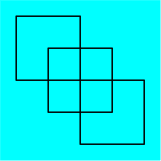
\includegraphics[width=0.25\linewidth]{3squares/3squares}
		\label{fig:3squares}
	\end{figure}
	\begin{figure}[H]
		\centering
		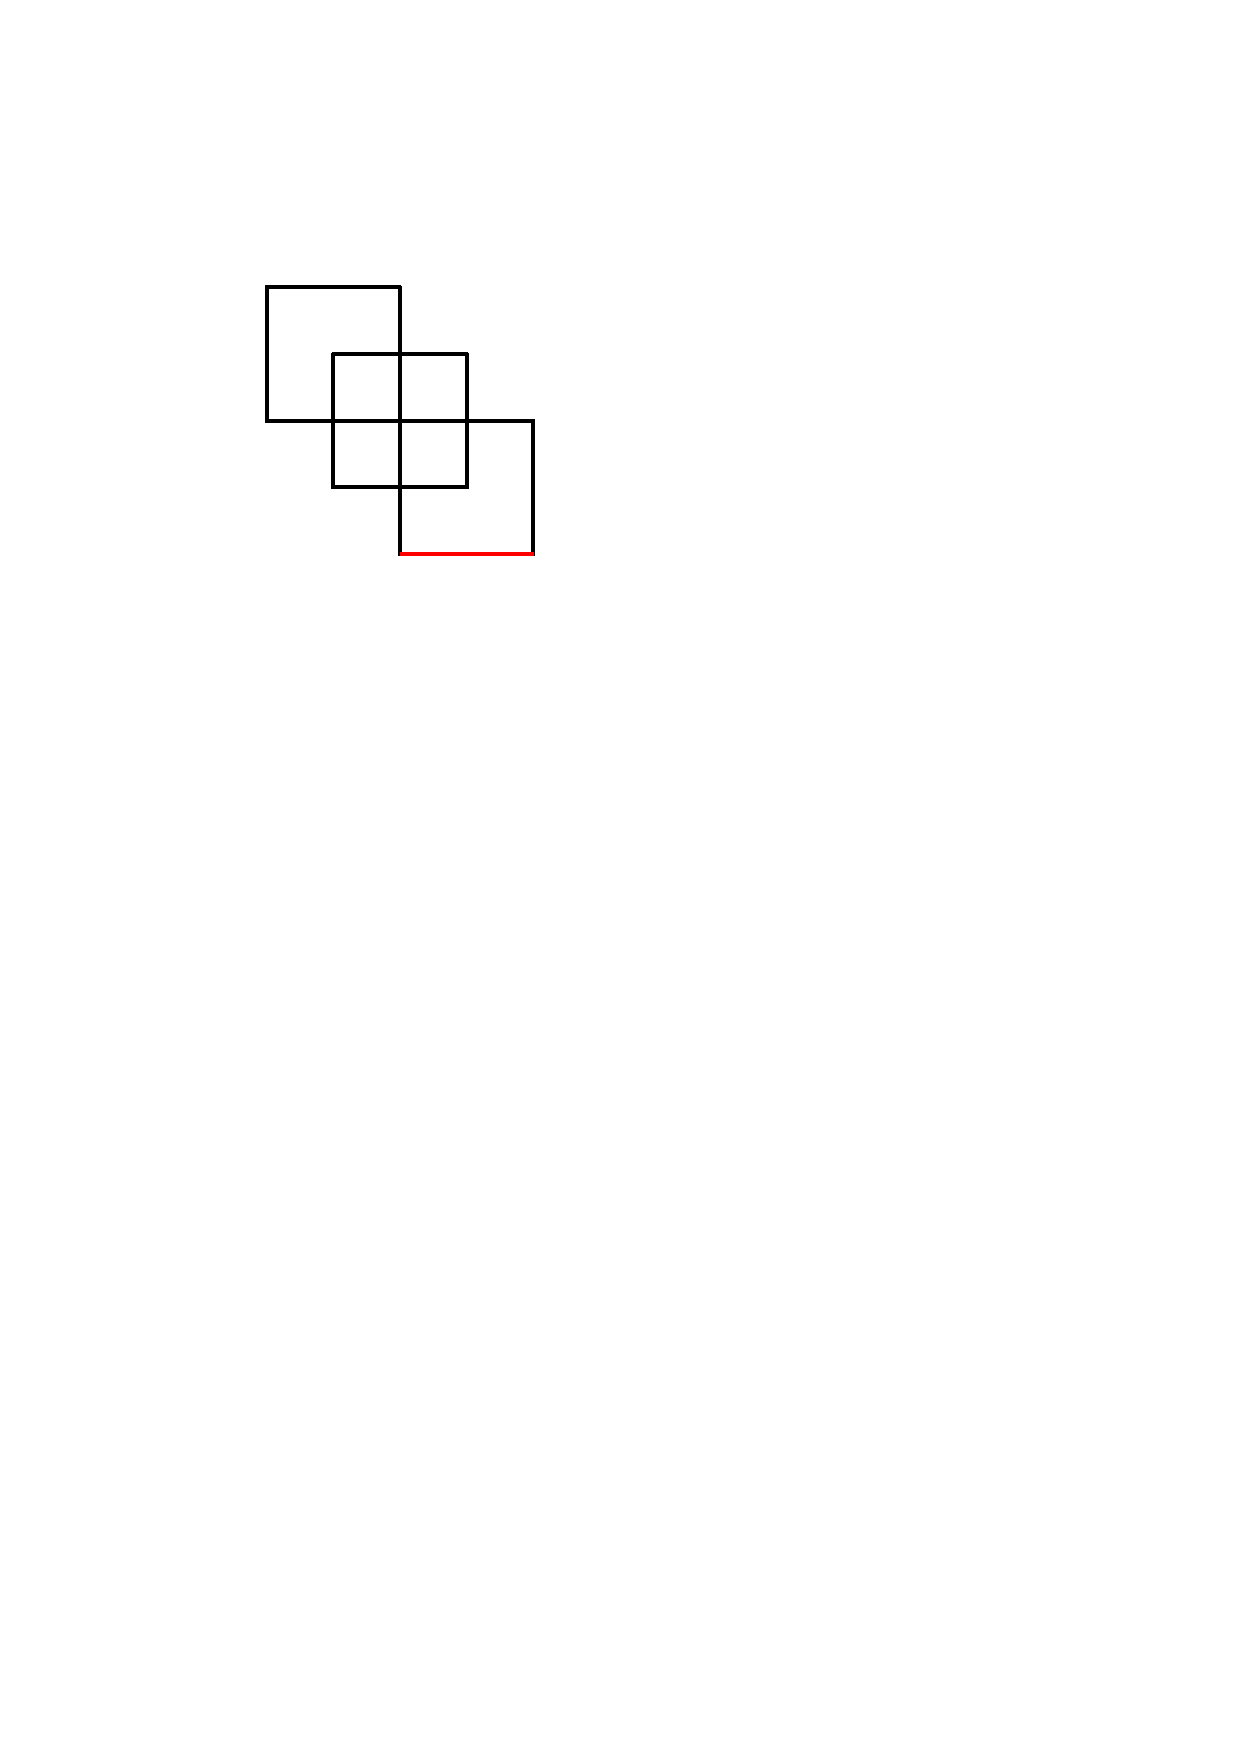
\includegraphics[width=0.25\linewidth]{3squares/3squares_pt1}
		\hspace{.05\linewidth}
		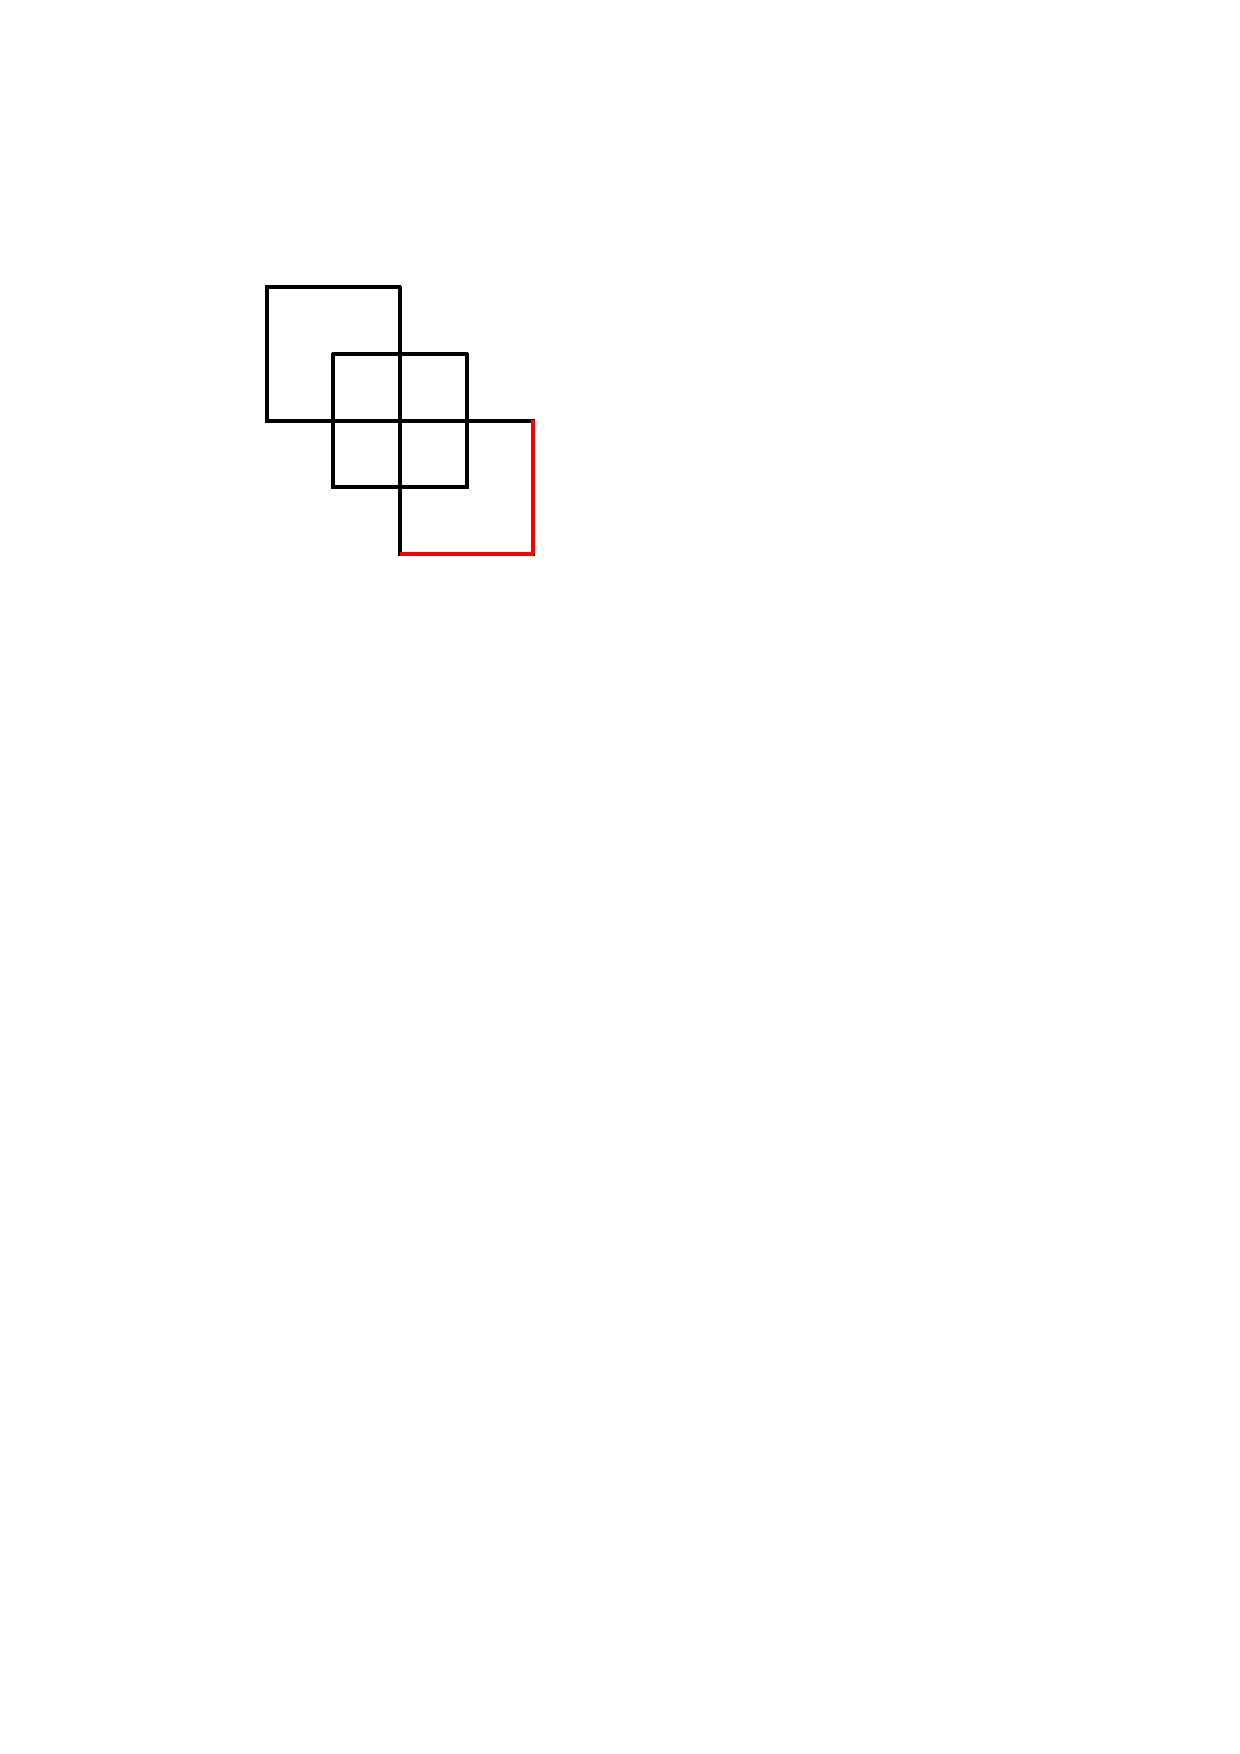
\includegraphics[width=0.25\linewidth]{3squares/3squares_pt2}
		\hspace{.05\linewidth}
		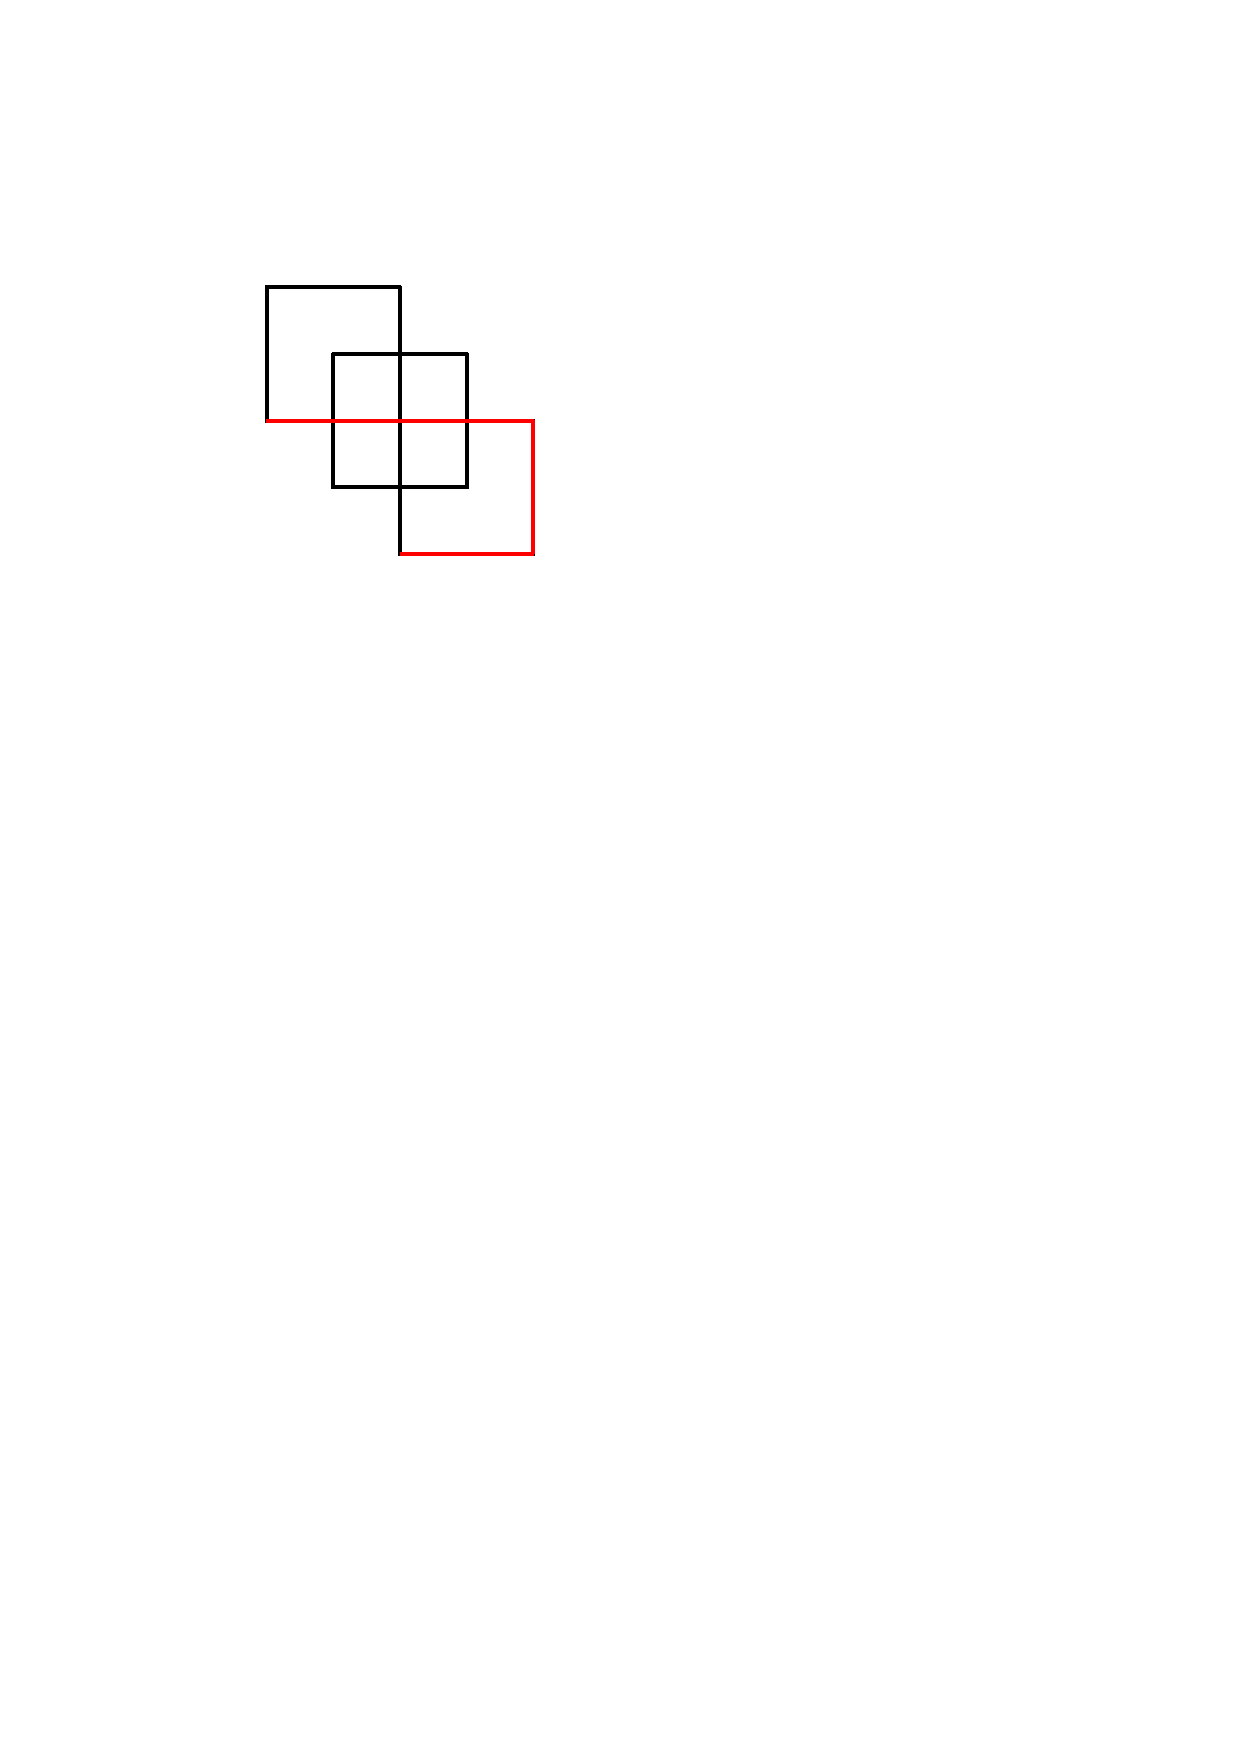
\includegraphics[width=0.25\linewidth]{3squares/3squares_pt3}
		\hspace{.05\linewidth}\\\vspace{1cm}
		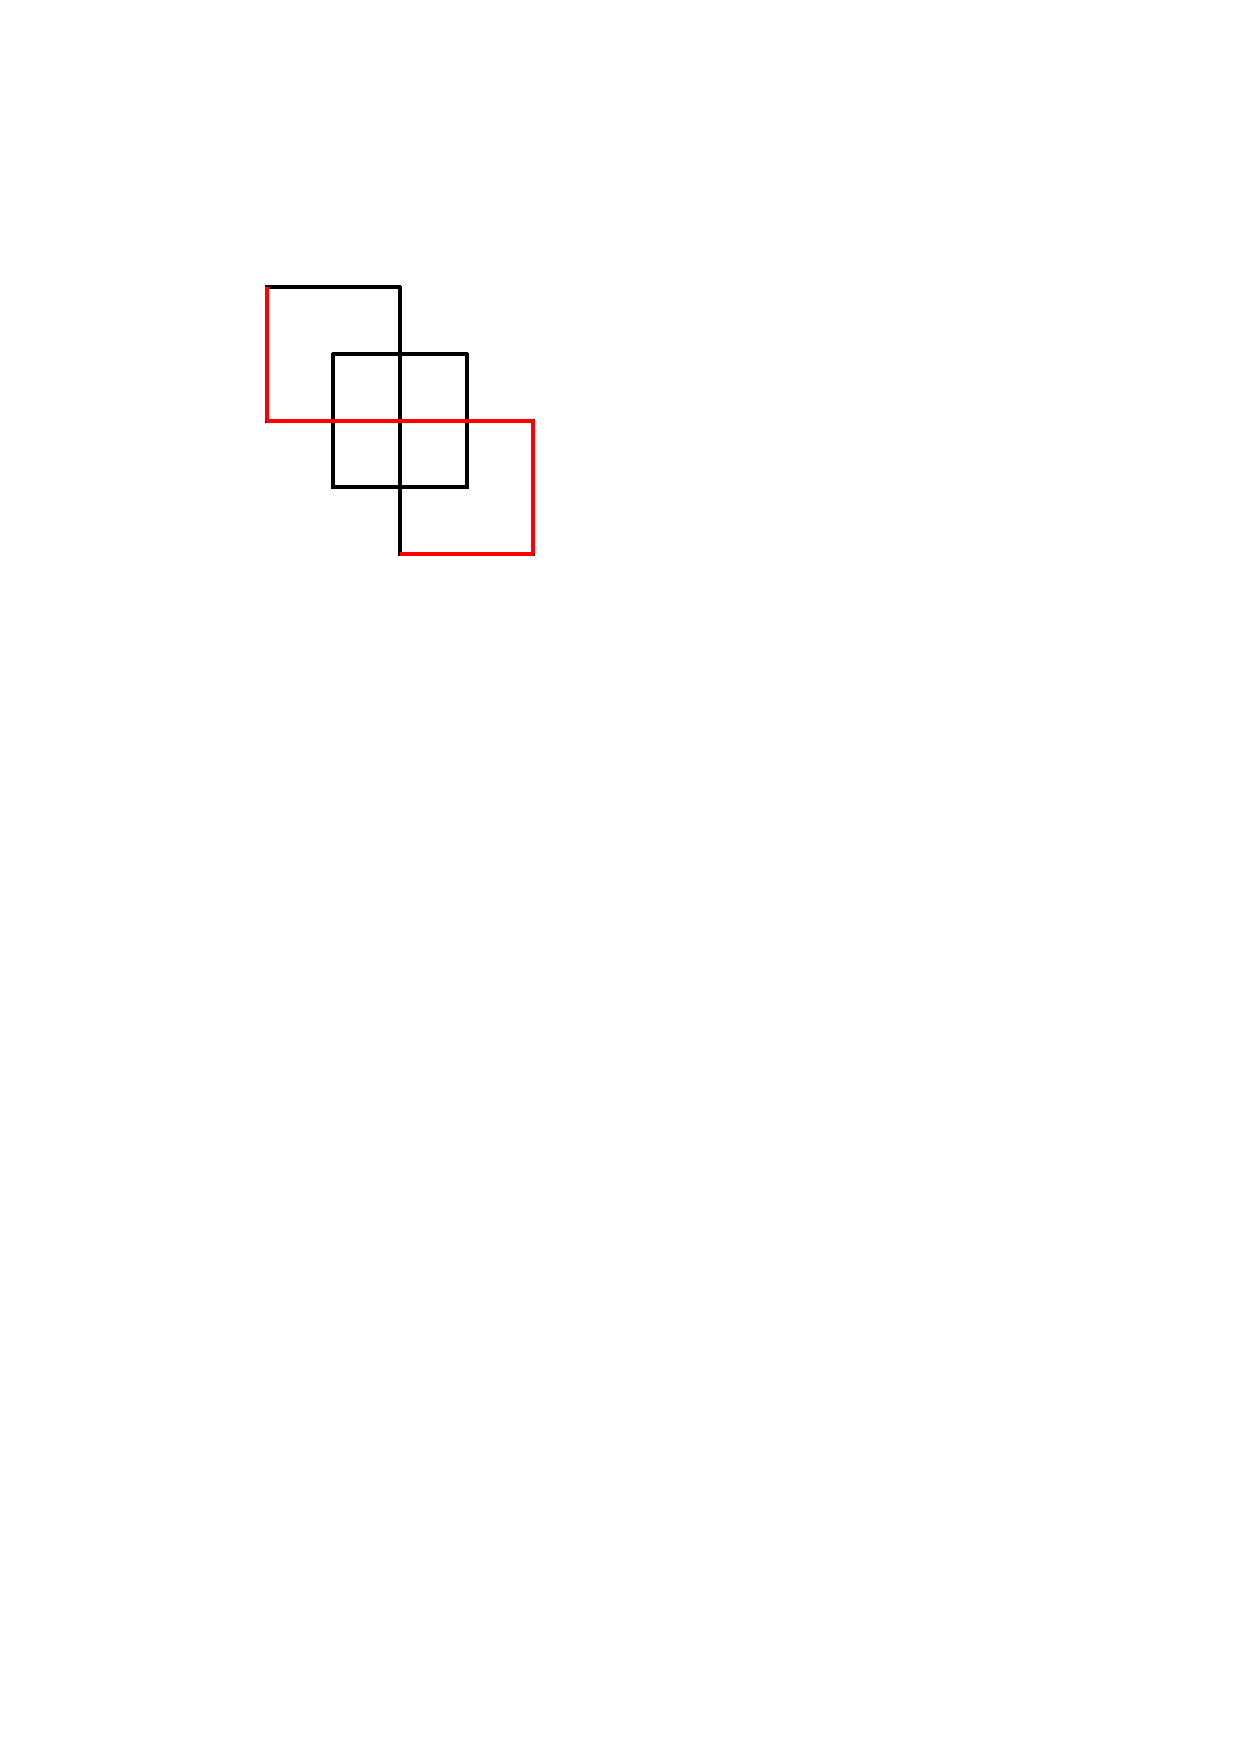
\includegraphics[width=0.25\linewidth]{3squares/3squares_pt4}
		\hspace{.05\linewidth}
		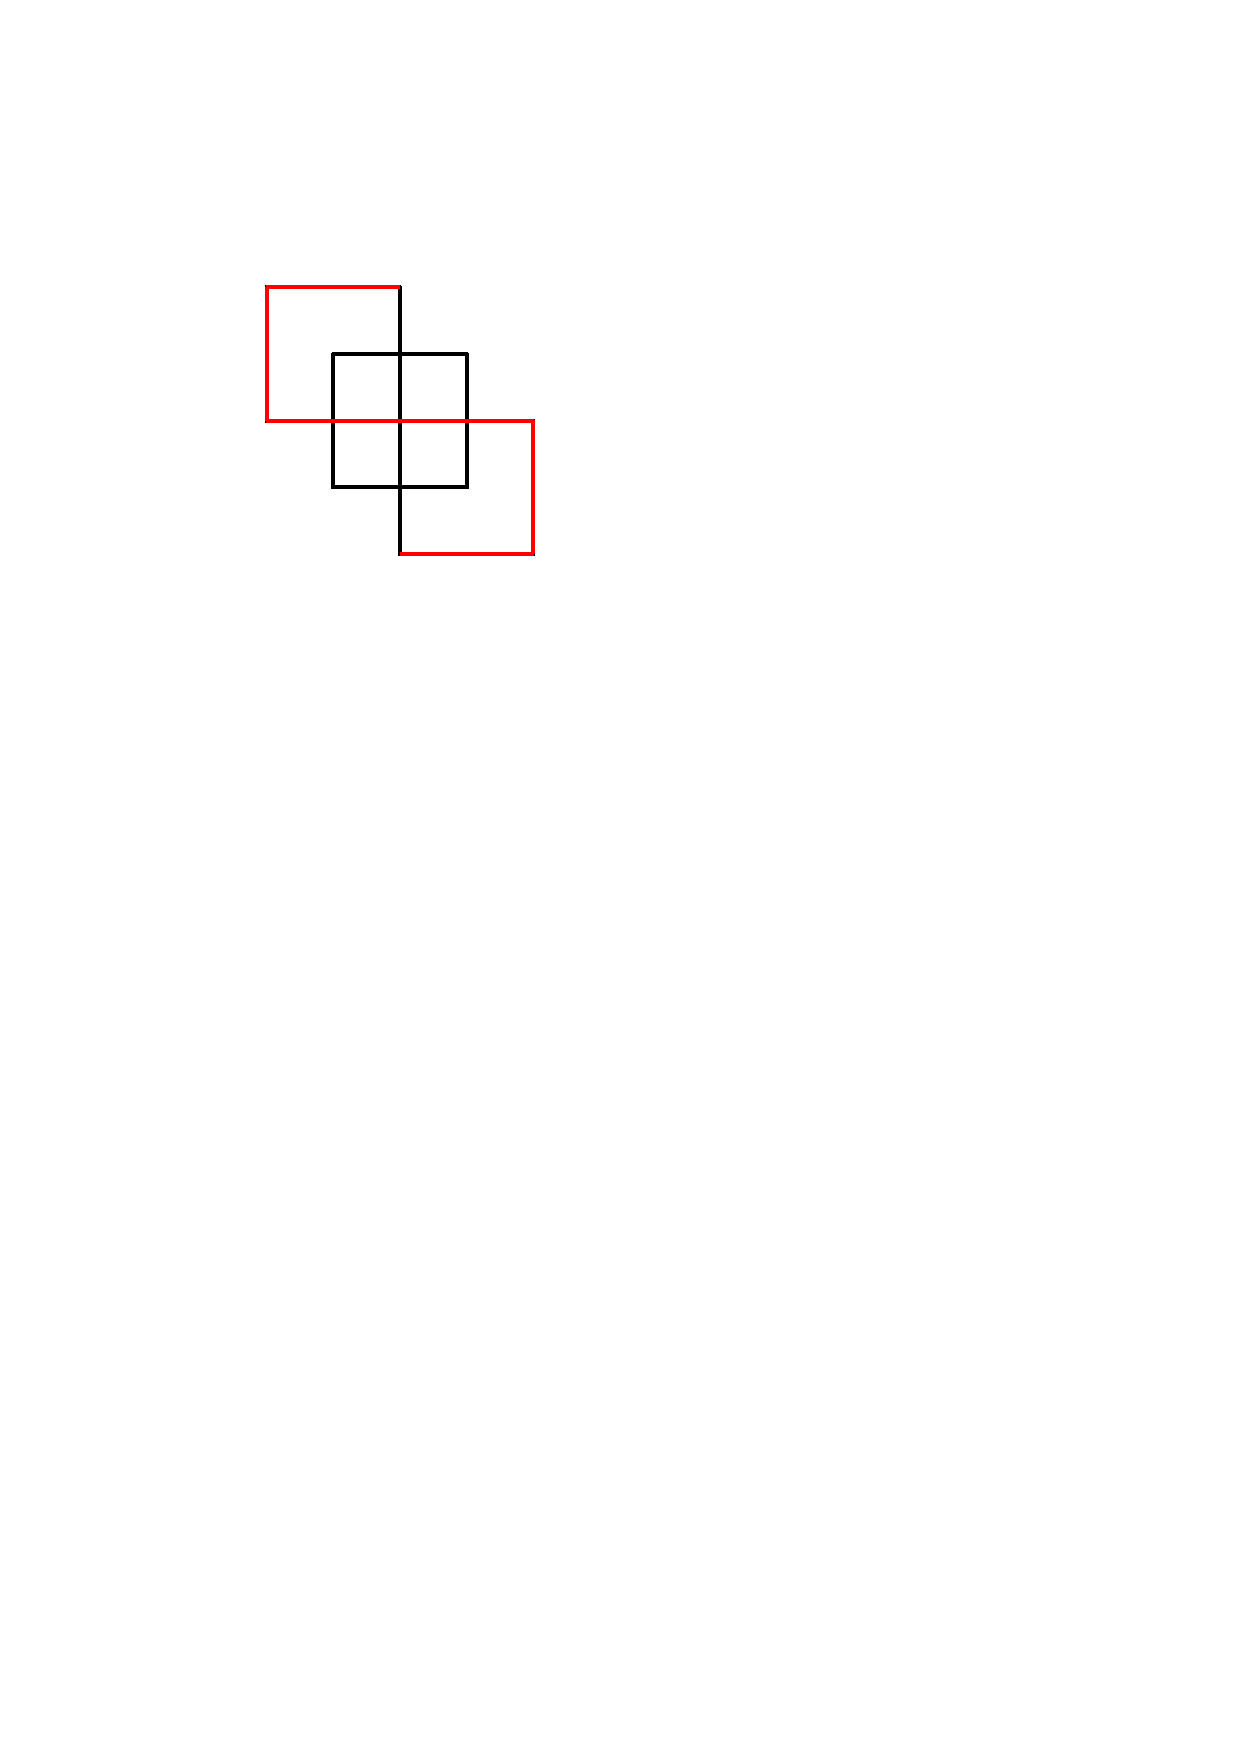
\includegraphics[width=0.25\linewidth]{3squares/3squares_pt5}
		\hspace{.05\linewidth}
		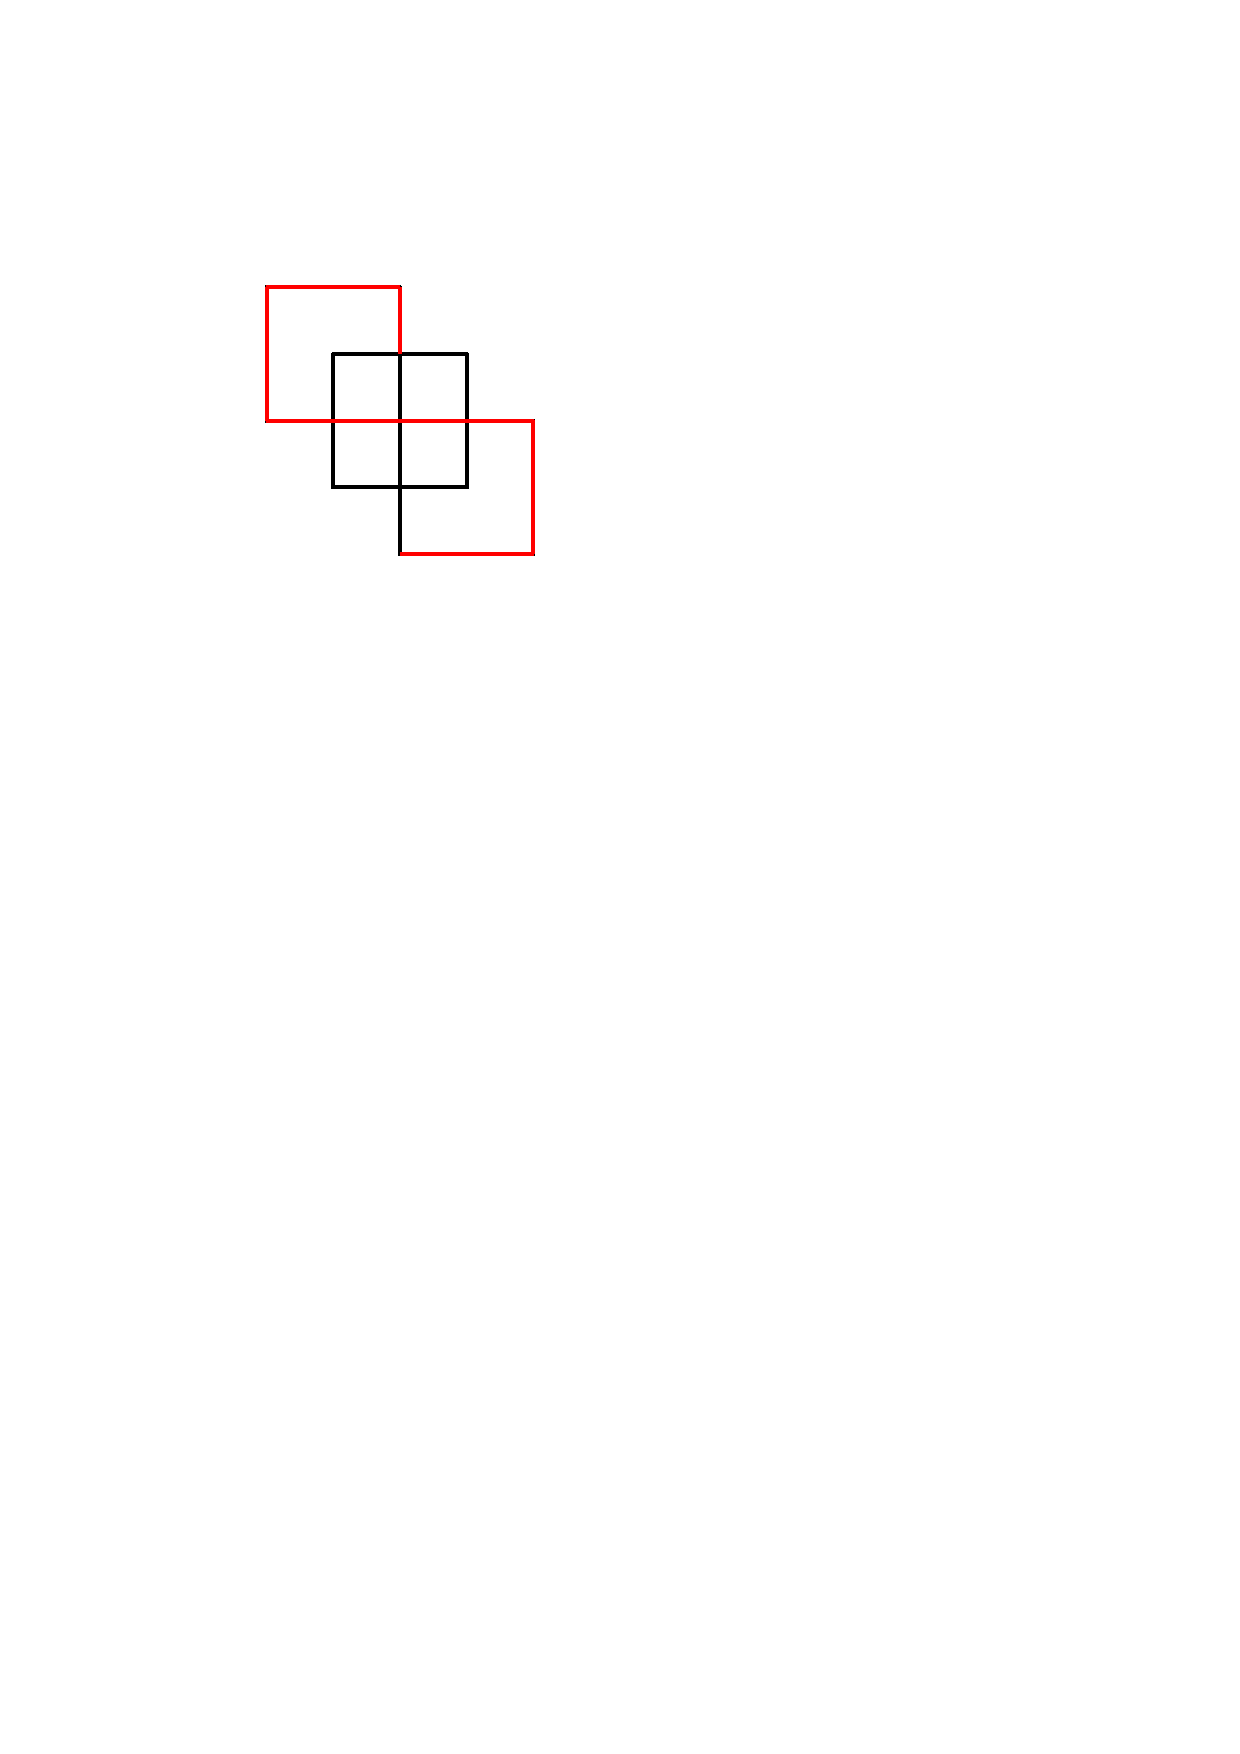
\includegraphics[width=0.25\linewidth]{3squares/3squares_pt6}
		\hspace{.05\linewidth}\\\vspace{1cm}
		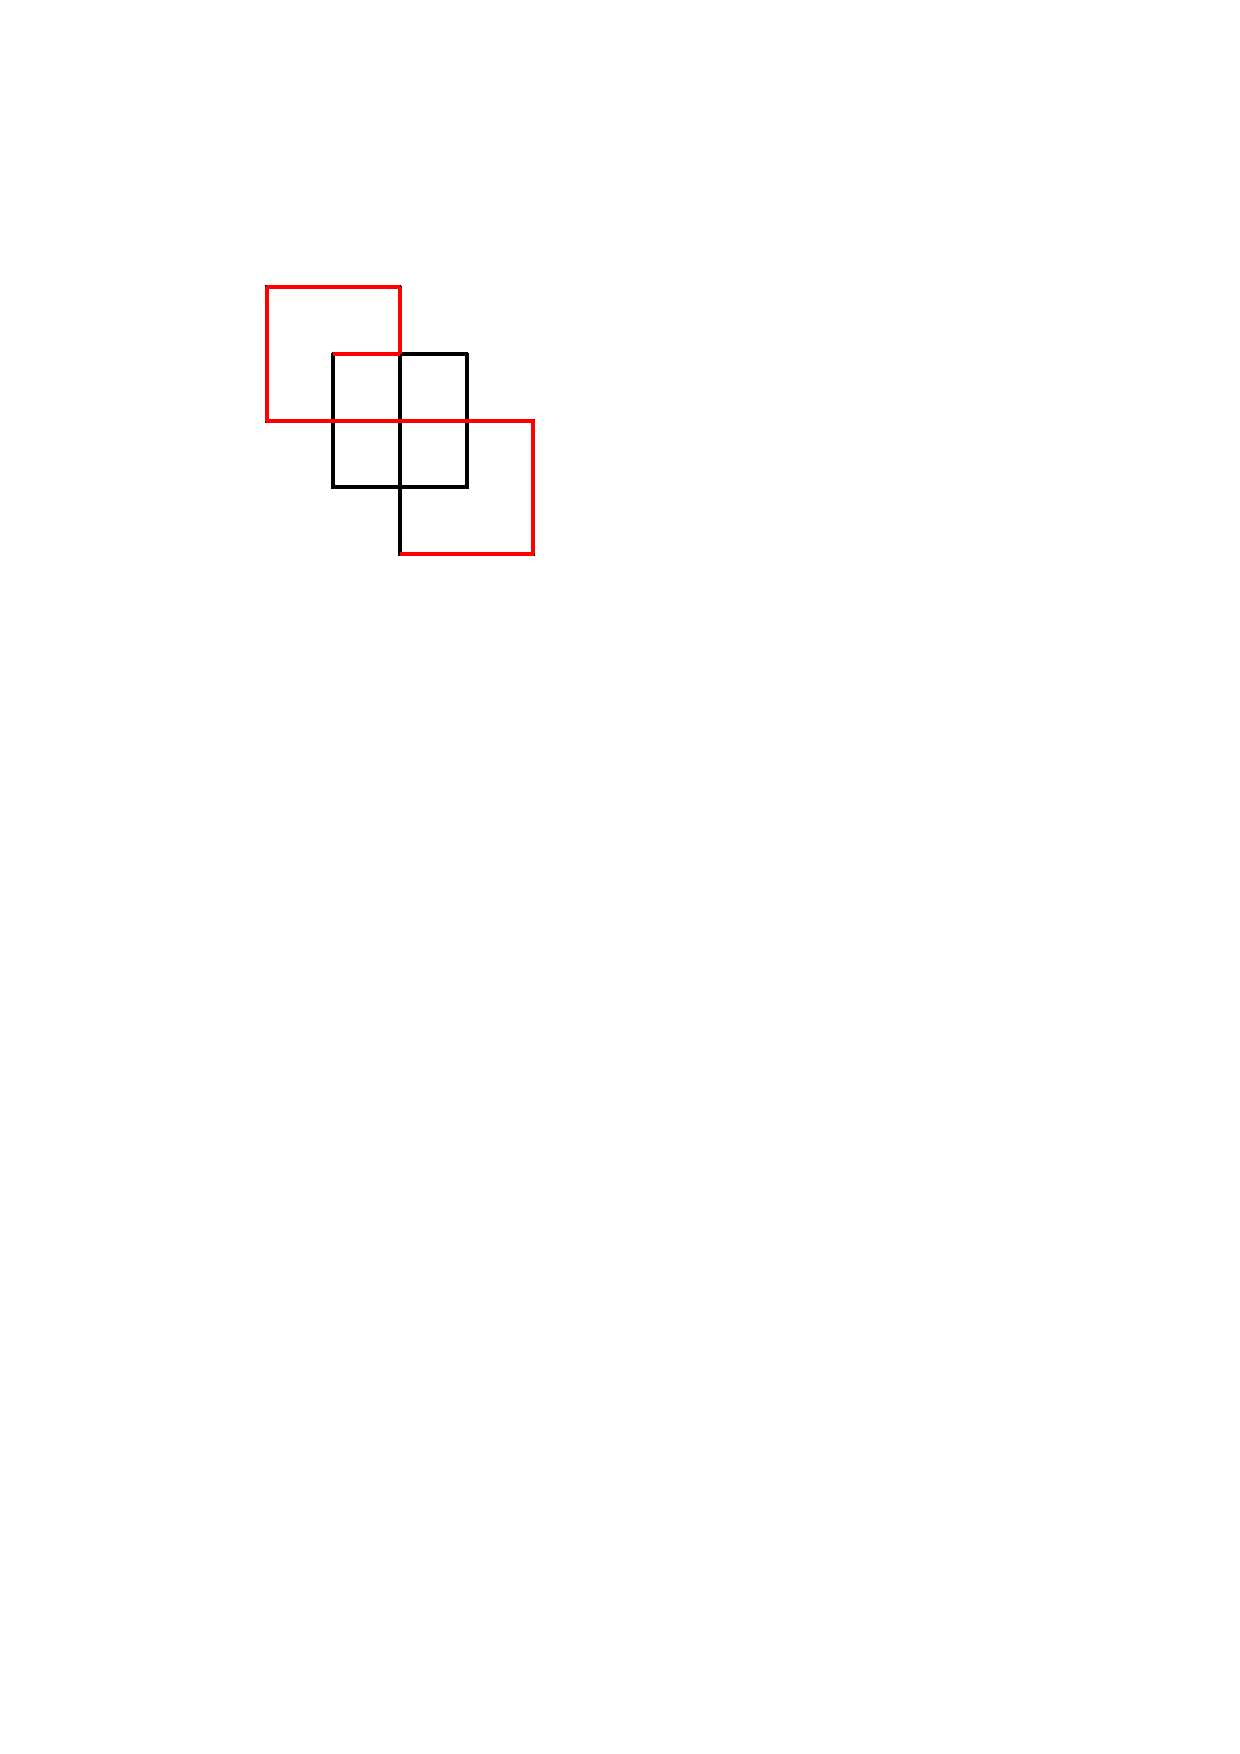
\includegraphics[width=0.25\linewidth]{3squares/3squares_pt7}
		\hspace{.05\linewidth}
		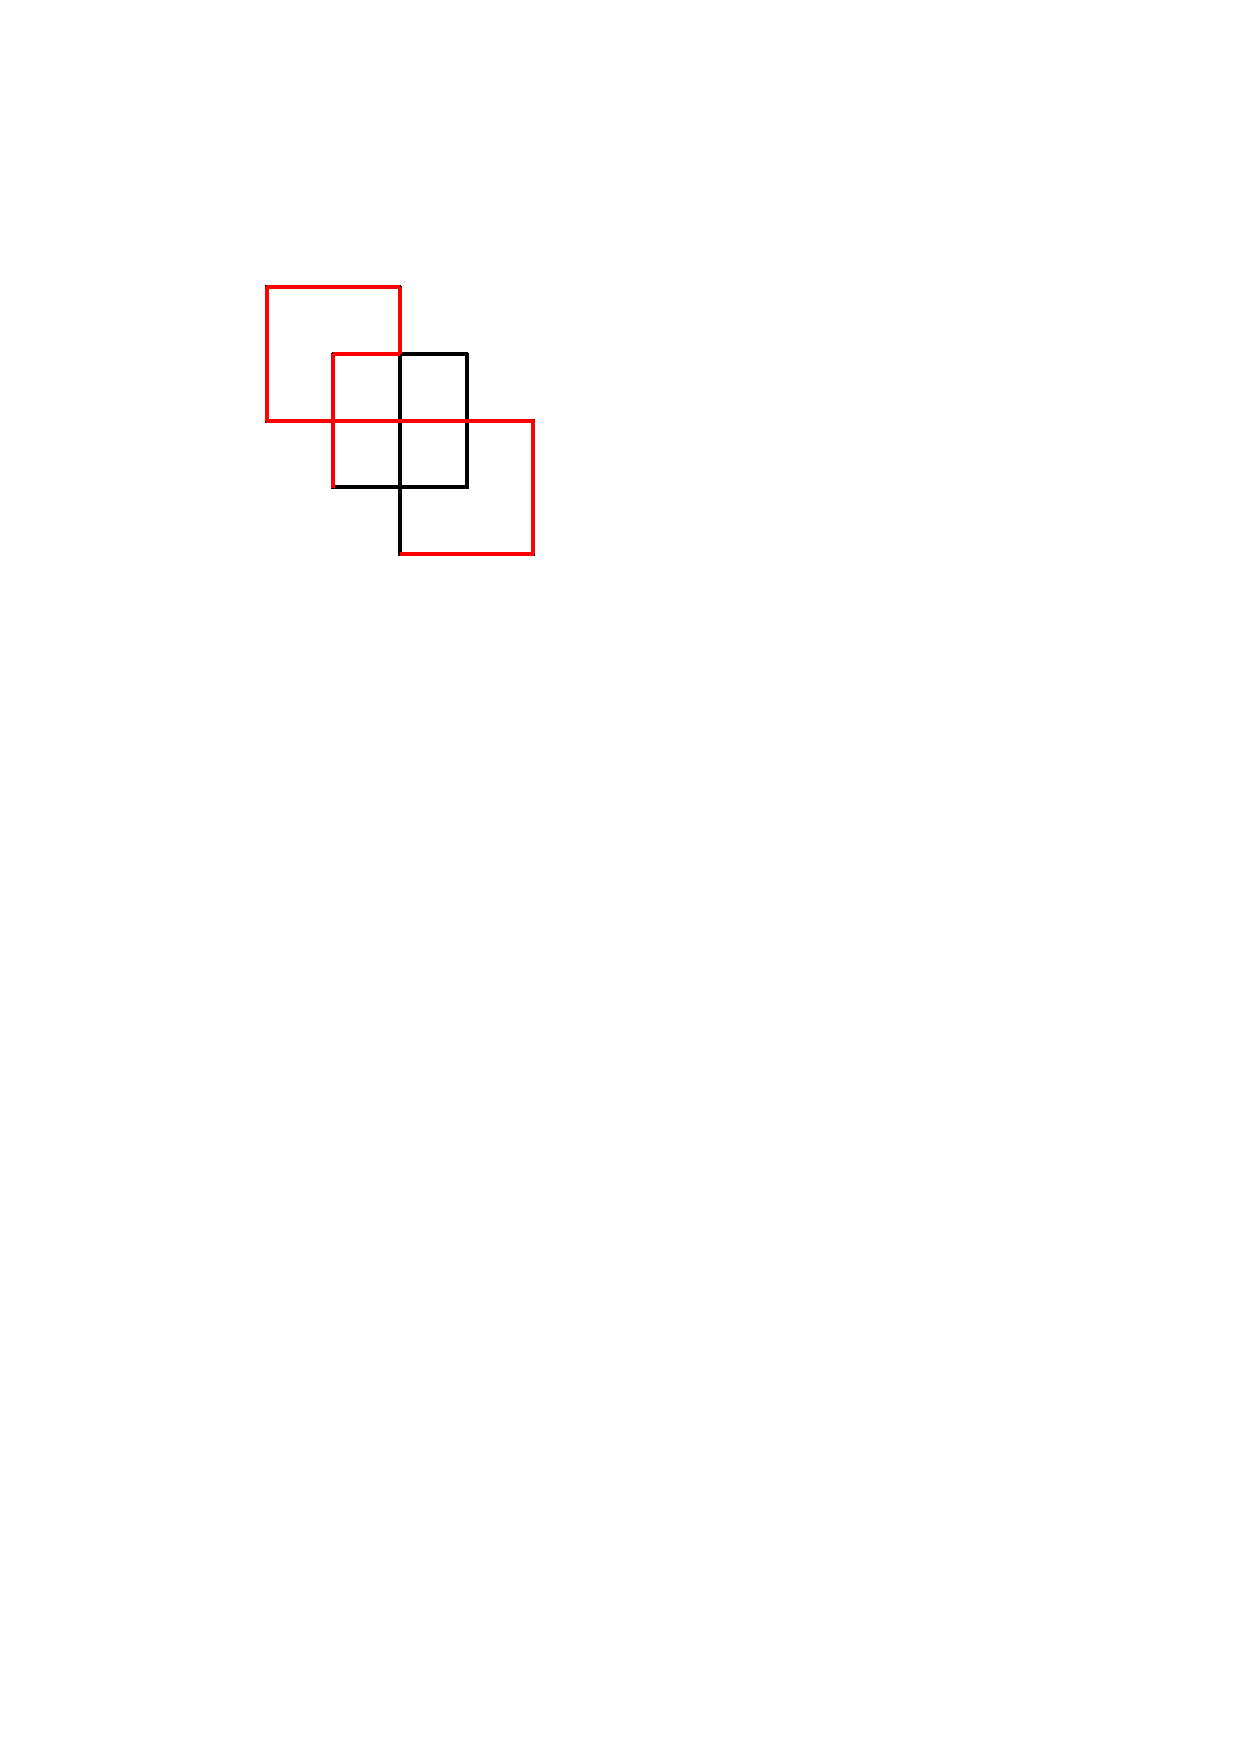
\includegraphics[width=0.25\linewidth]{3squares/3squares_pt8}
		\hspace{.05\linewidth}
		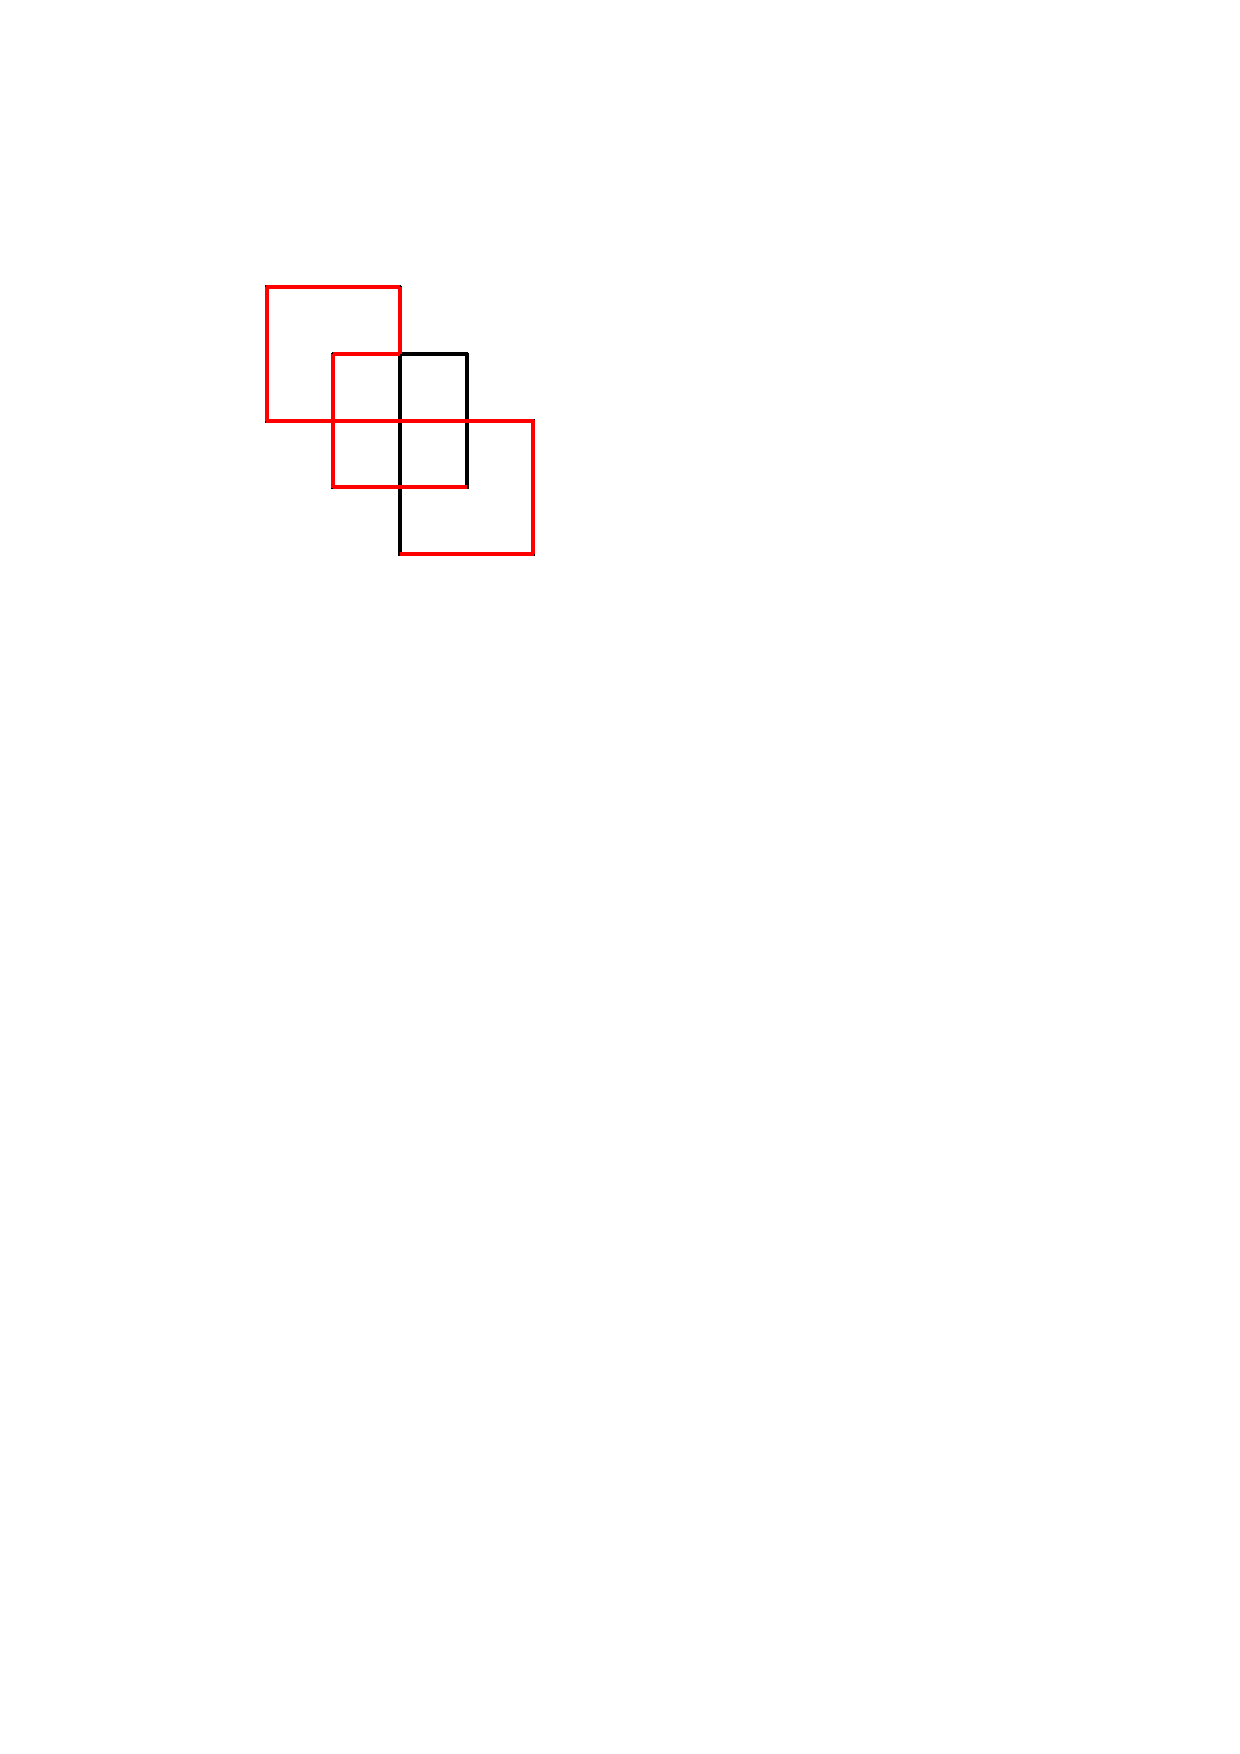
\includegraphics[width=0.25\linewidth]{3squares/3squares_pt9}
		\hspace{.05\linewidth}\\\vspace{1cm}
		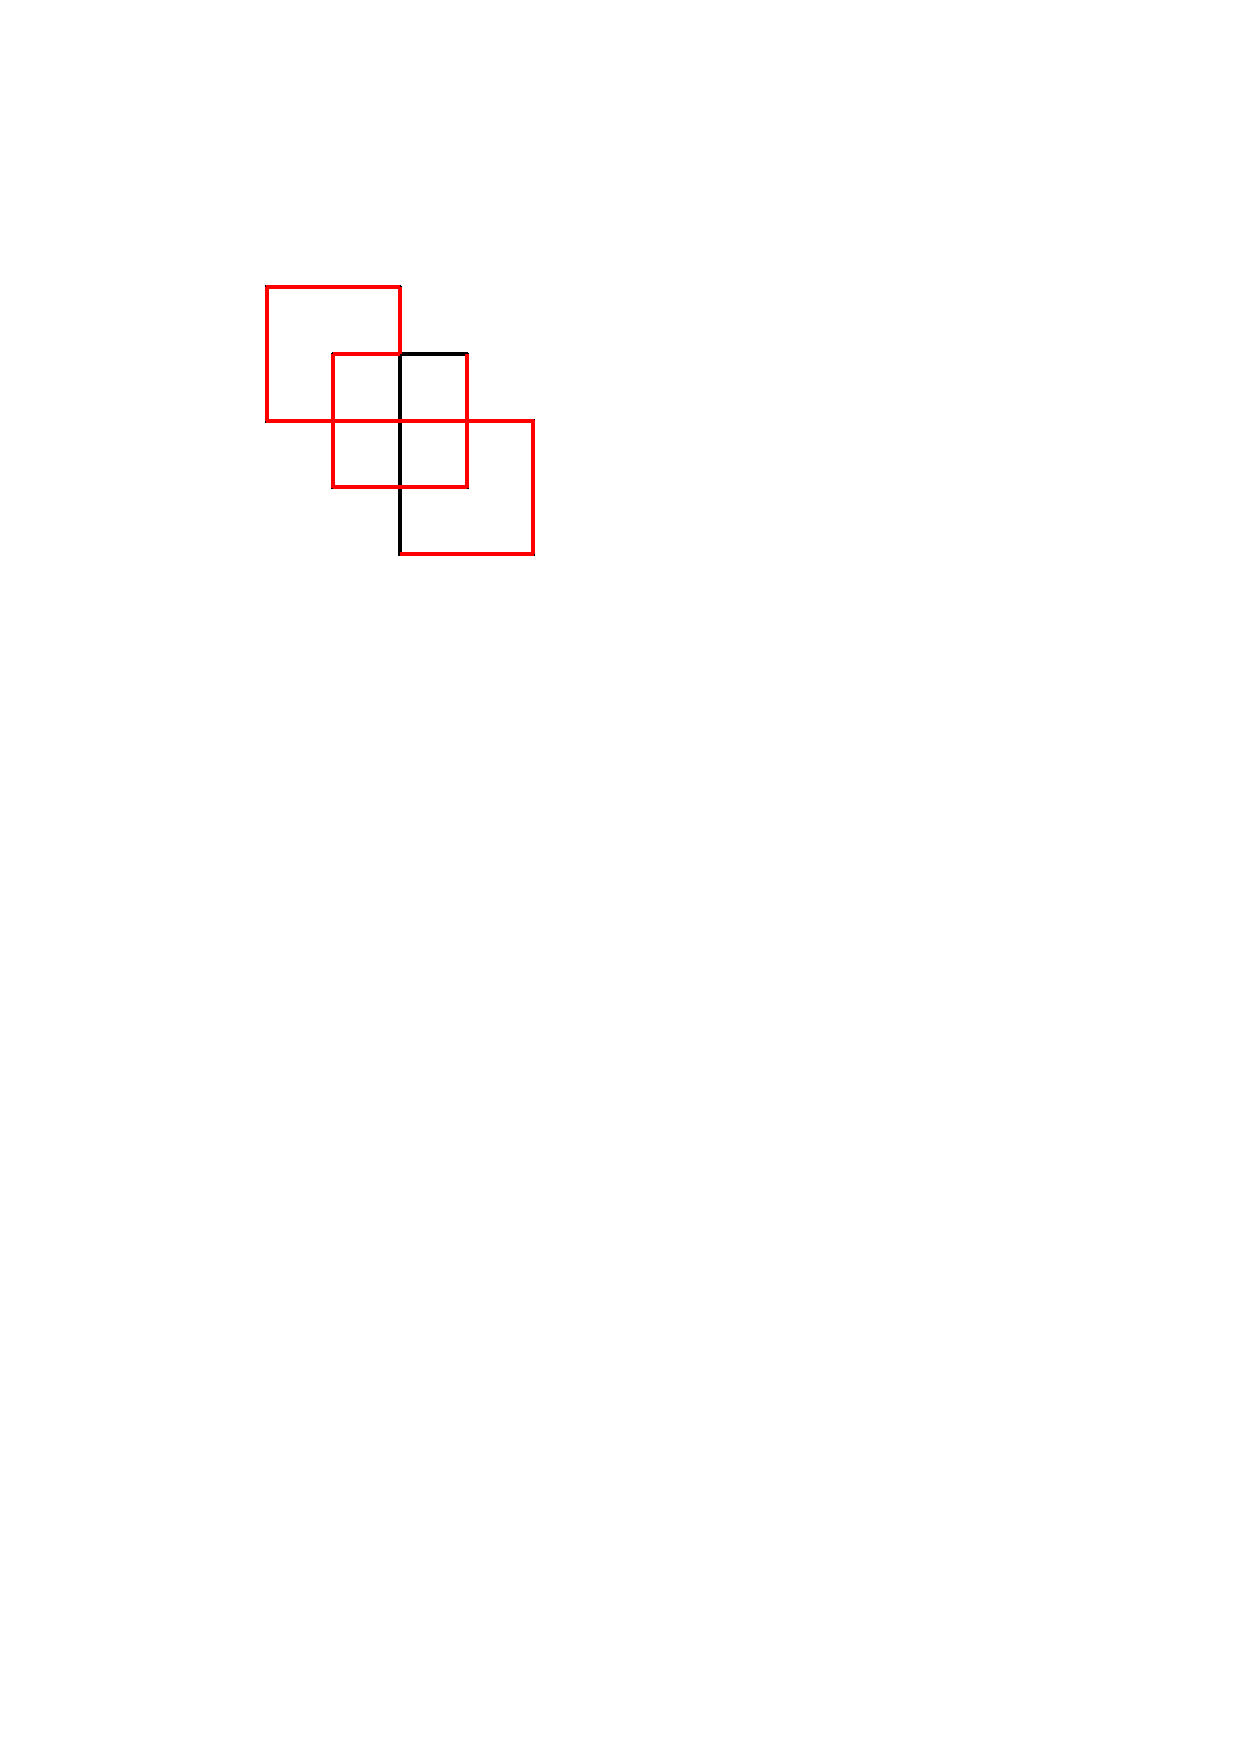
\includegraphics[width=0.25\linewidth]{3squares/3squares_pt10}
		\hspace{.05\linewidth}
		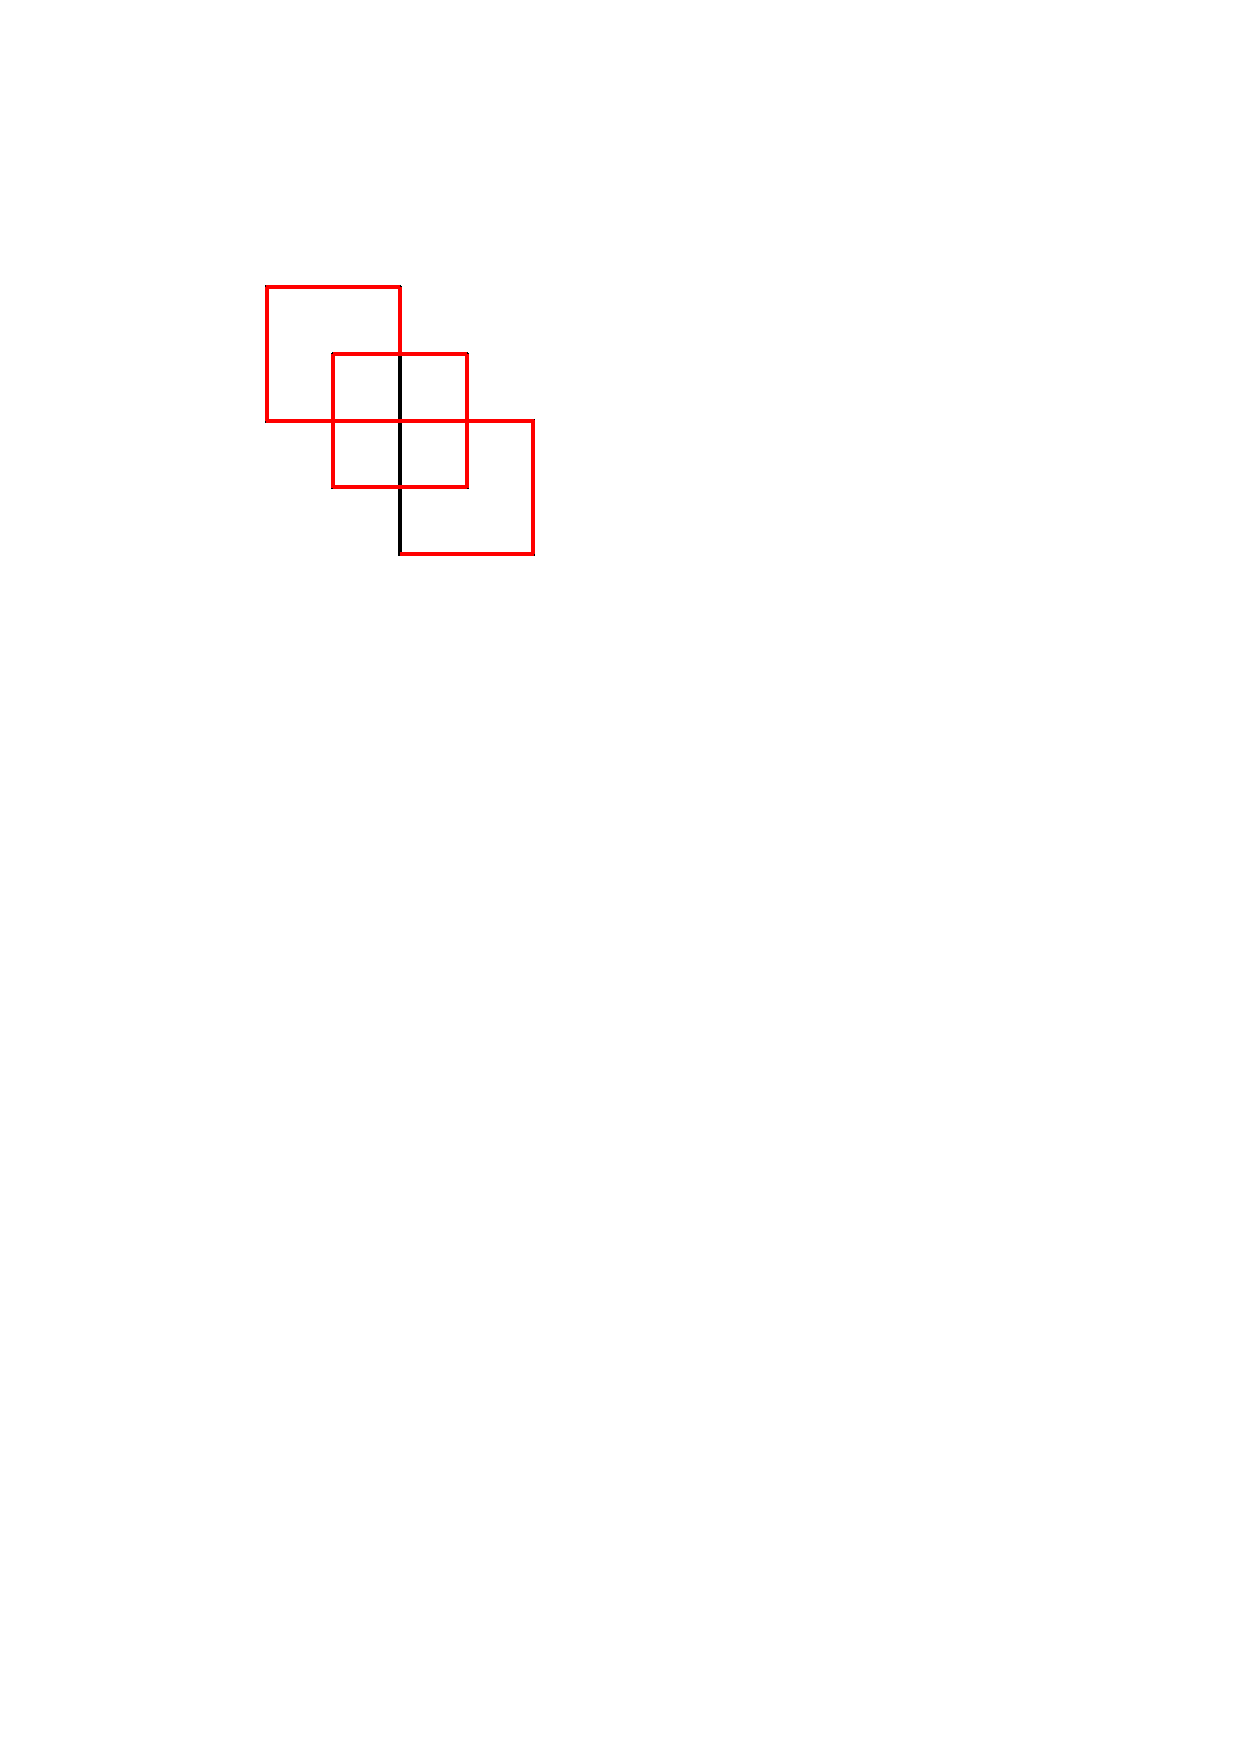
\includegraphics[width=0.25\linewidth]{3squares/3squares_pt11}
		\hspace{.05\linewidth}
		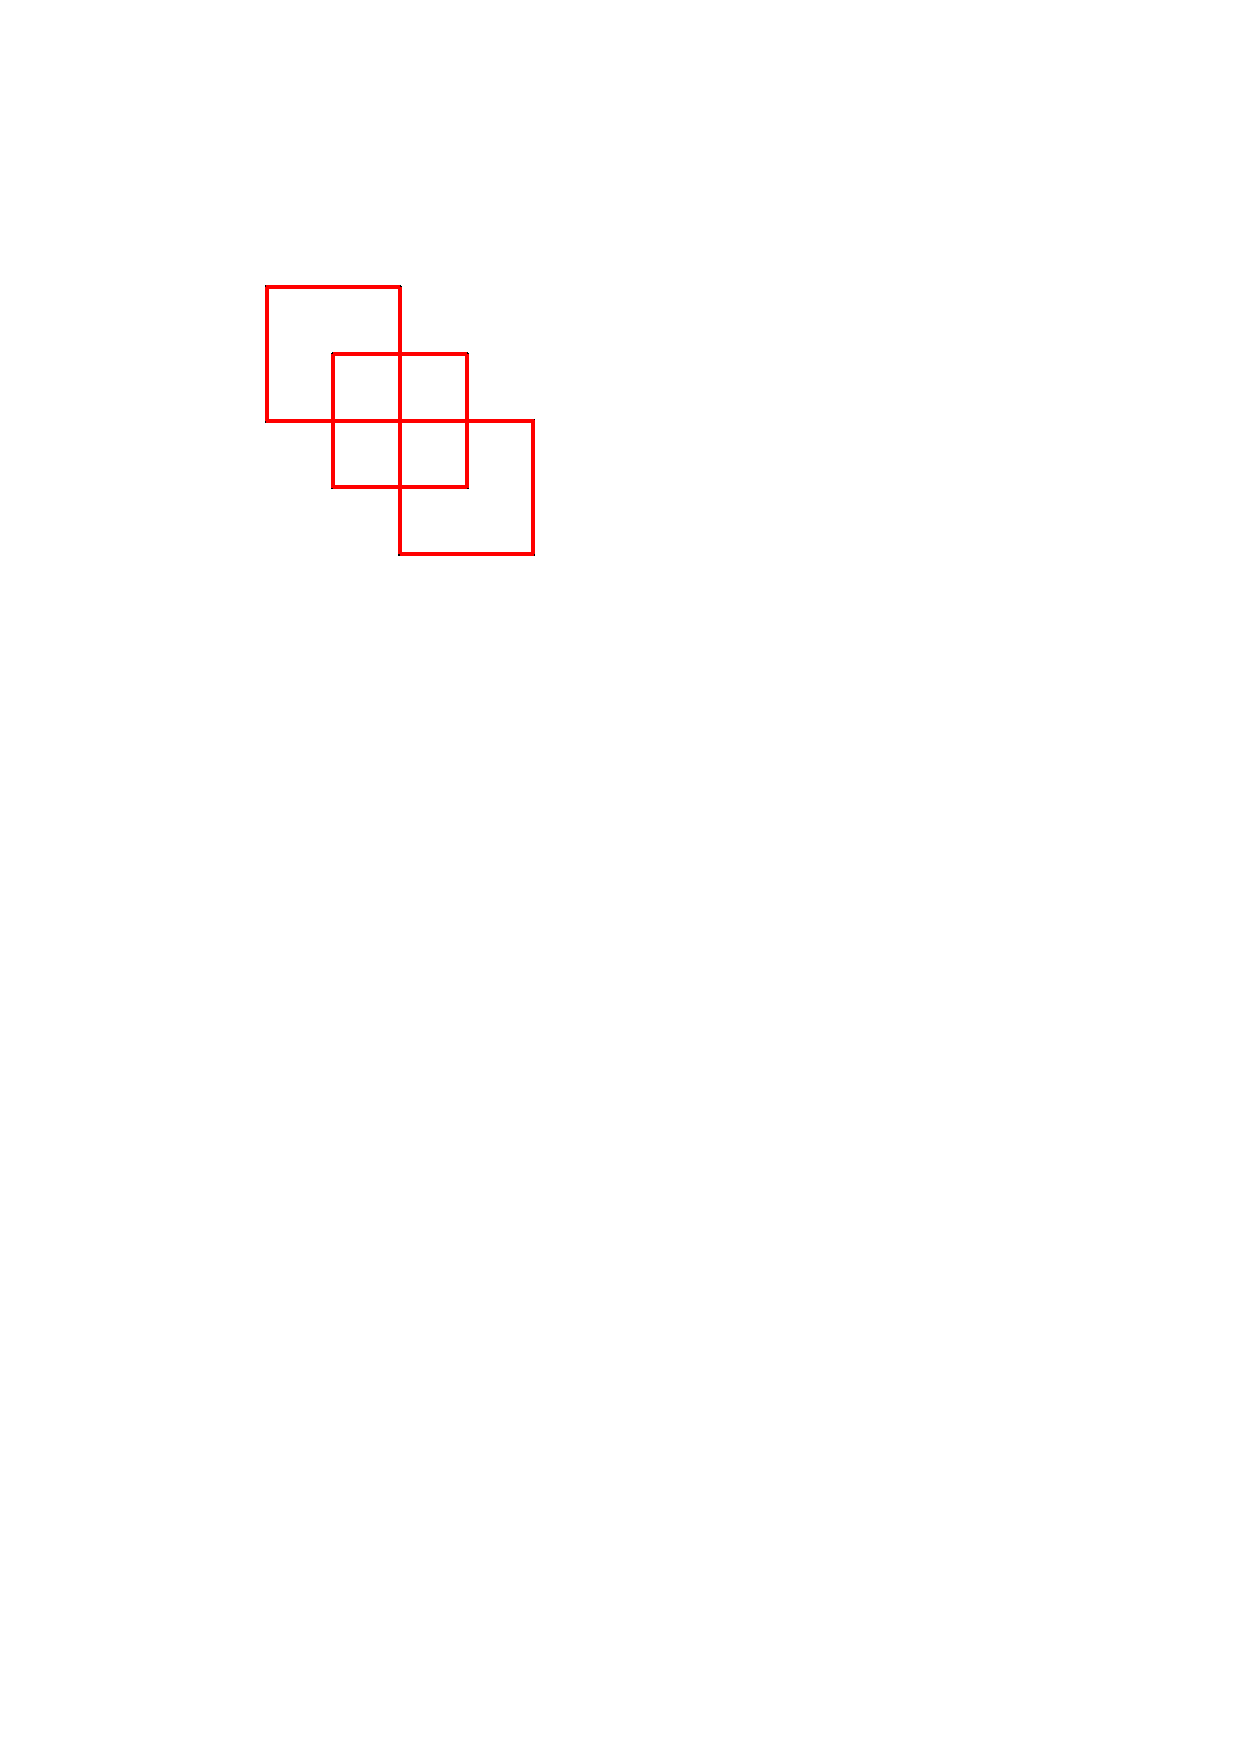
\includegraphics[width=0.25\linewidth]{3squares/3squares_pt12}
		\label{fig:3squarespt1}
	\end{figure}
	\newpage
	\section{O Olho de Sauron}
	\begin{figure}[H]
		\centering
		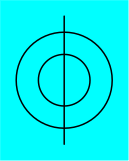
\includegraphics[width=0.3\linewidth]{sauron_s_eye/eye}
		\label{fig:eye}
	\end{figure}
	\begin{figure}[H]
		\centering
		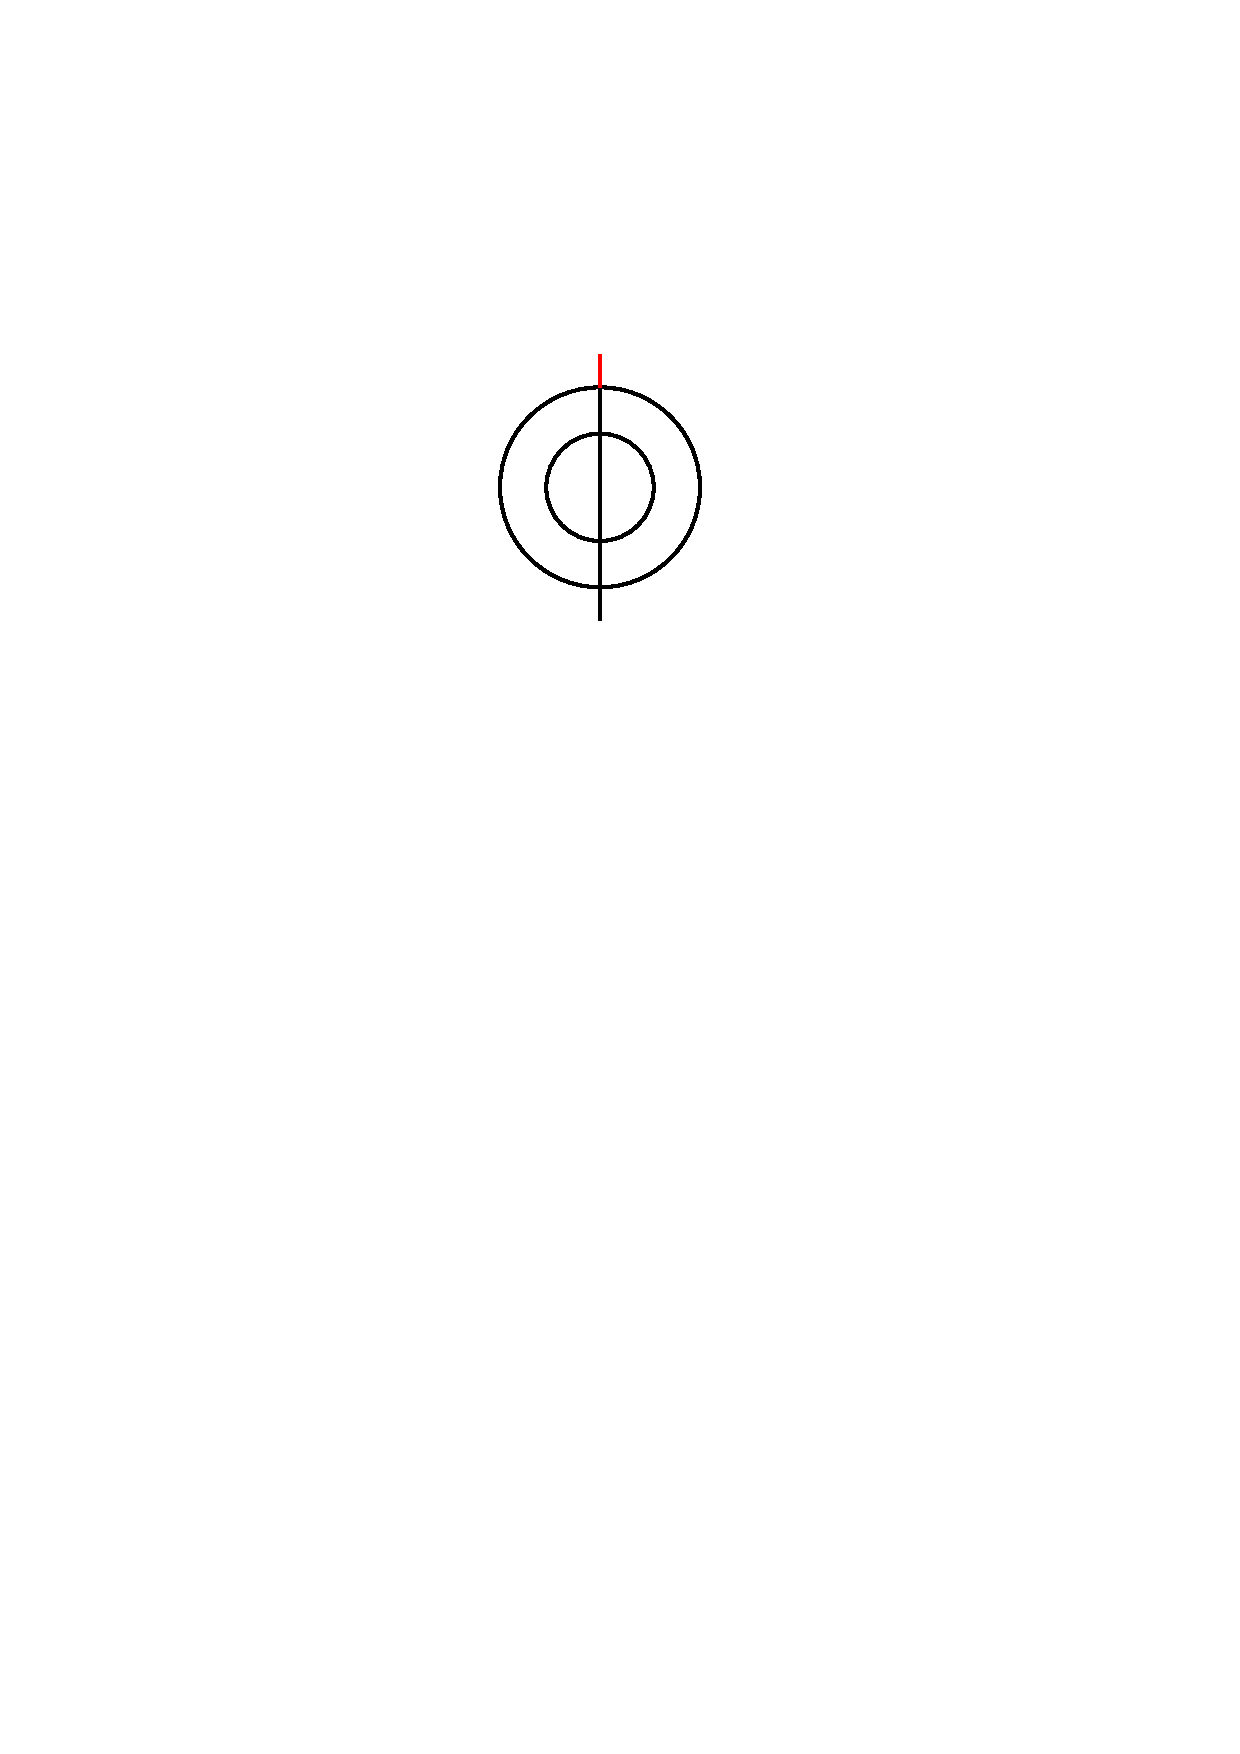
\includegraphics[width=0.25\linewidth]{sauron_s_eye/eye_pt1}
		\hspace{.05\linewidth}
		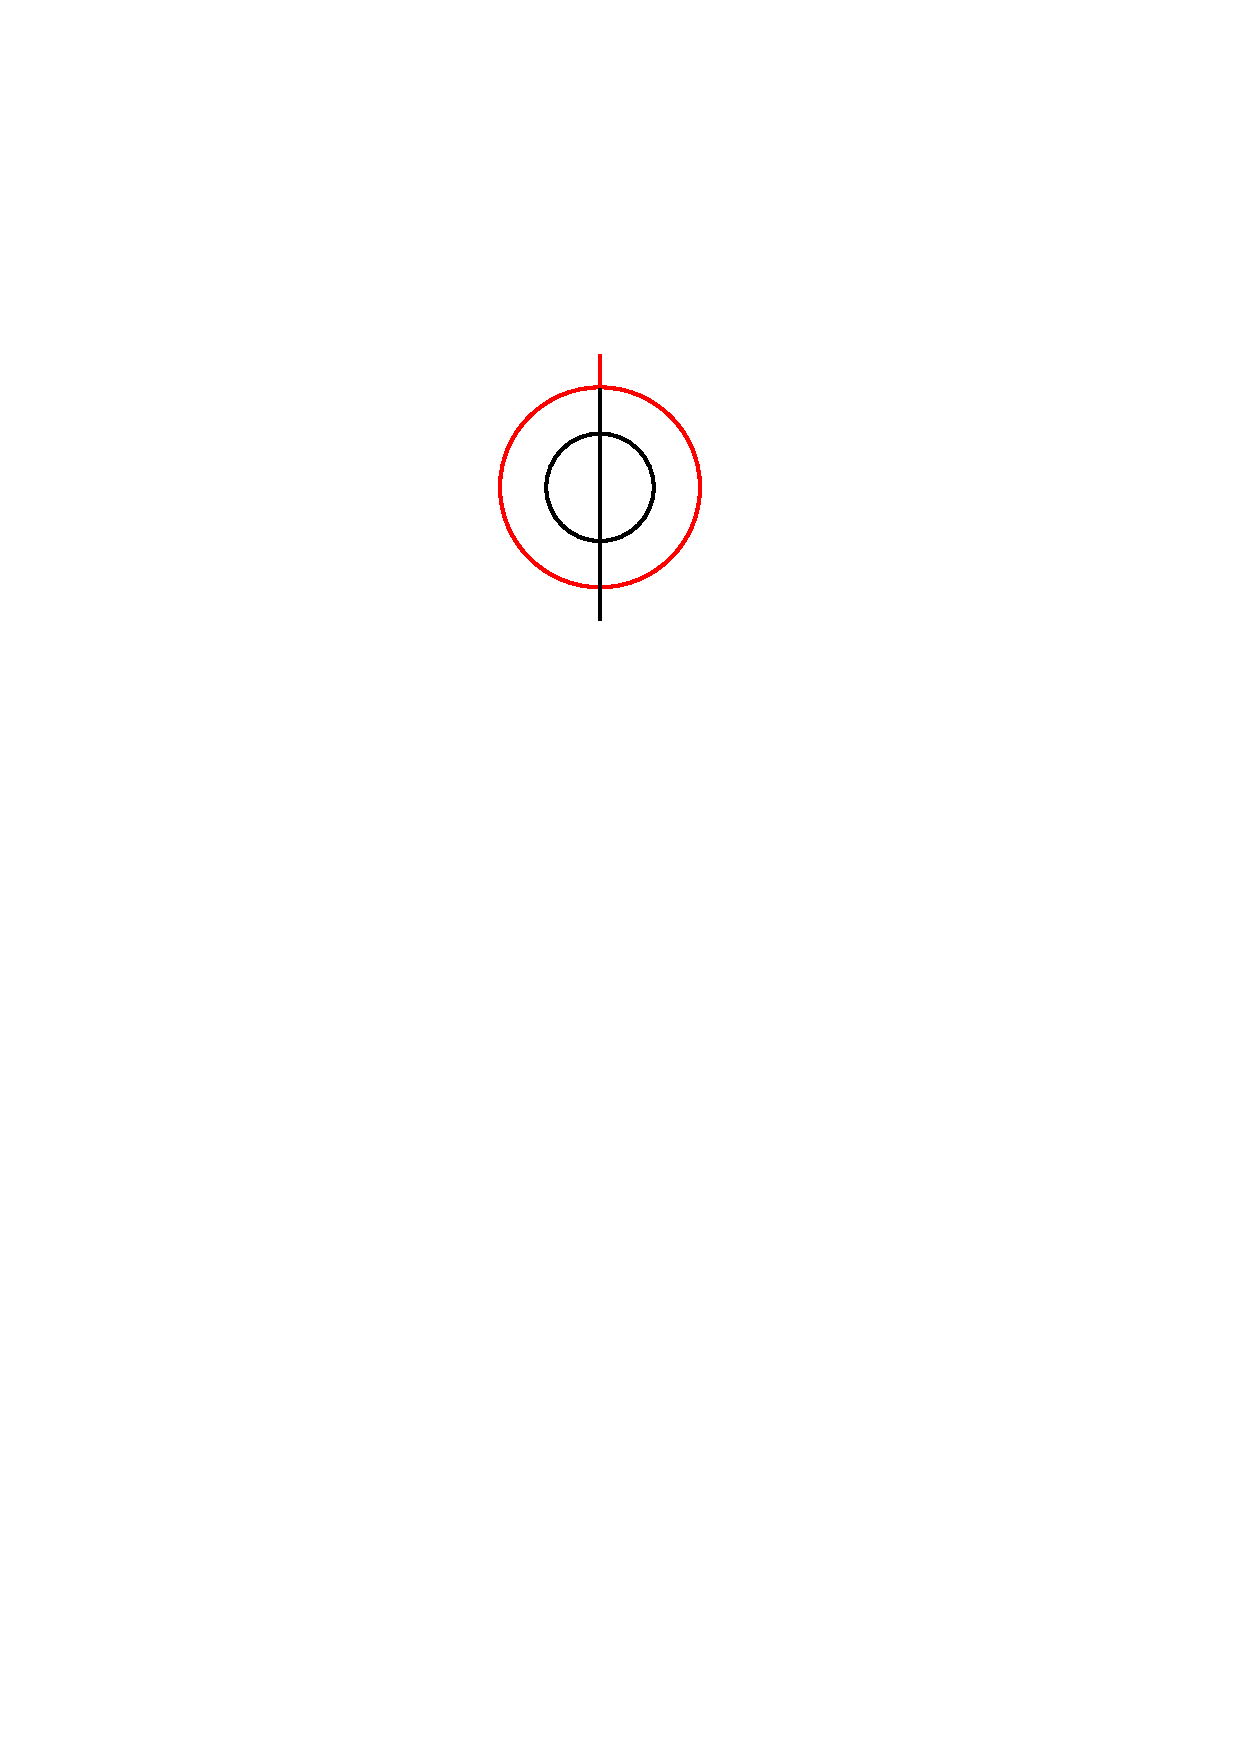
\includegraphics[width=0.25\linewidth]{sauron_s_eye/eye_pt2}
		\hspace{.05\linewidth}
		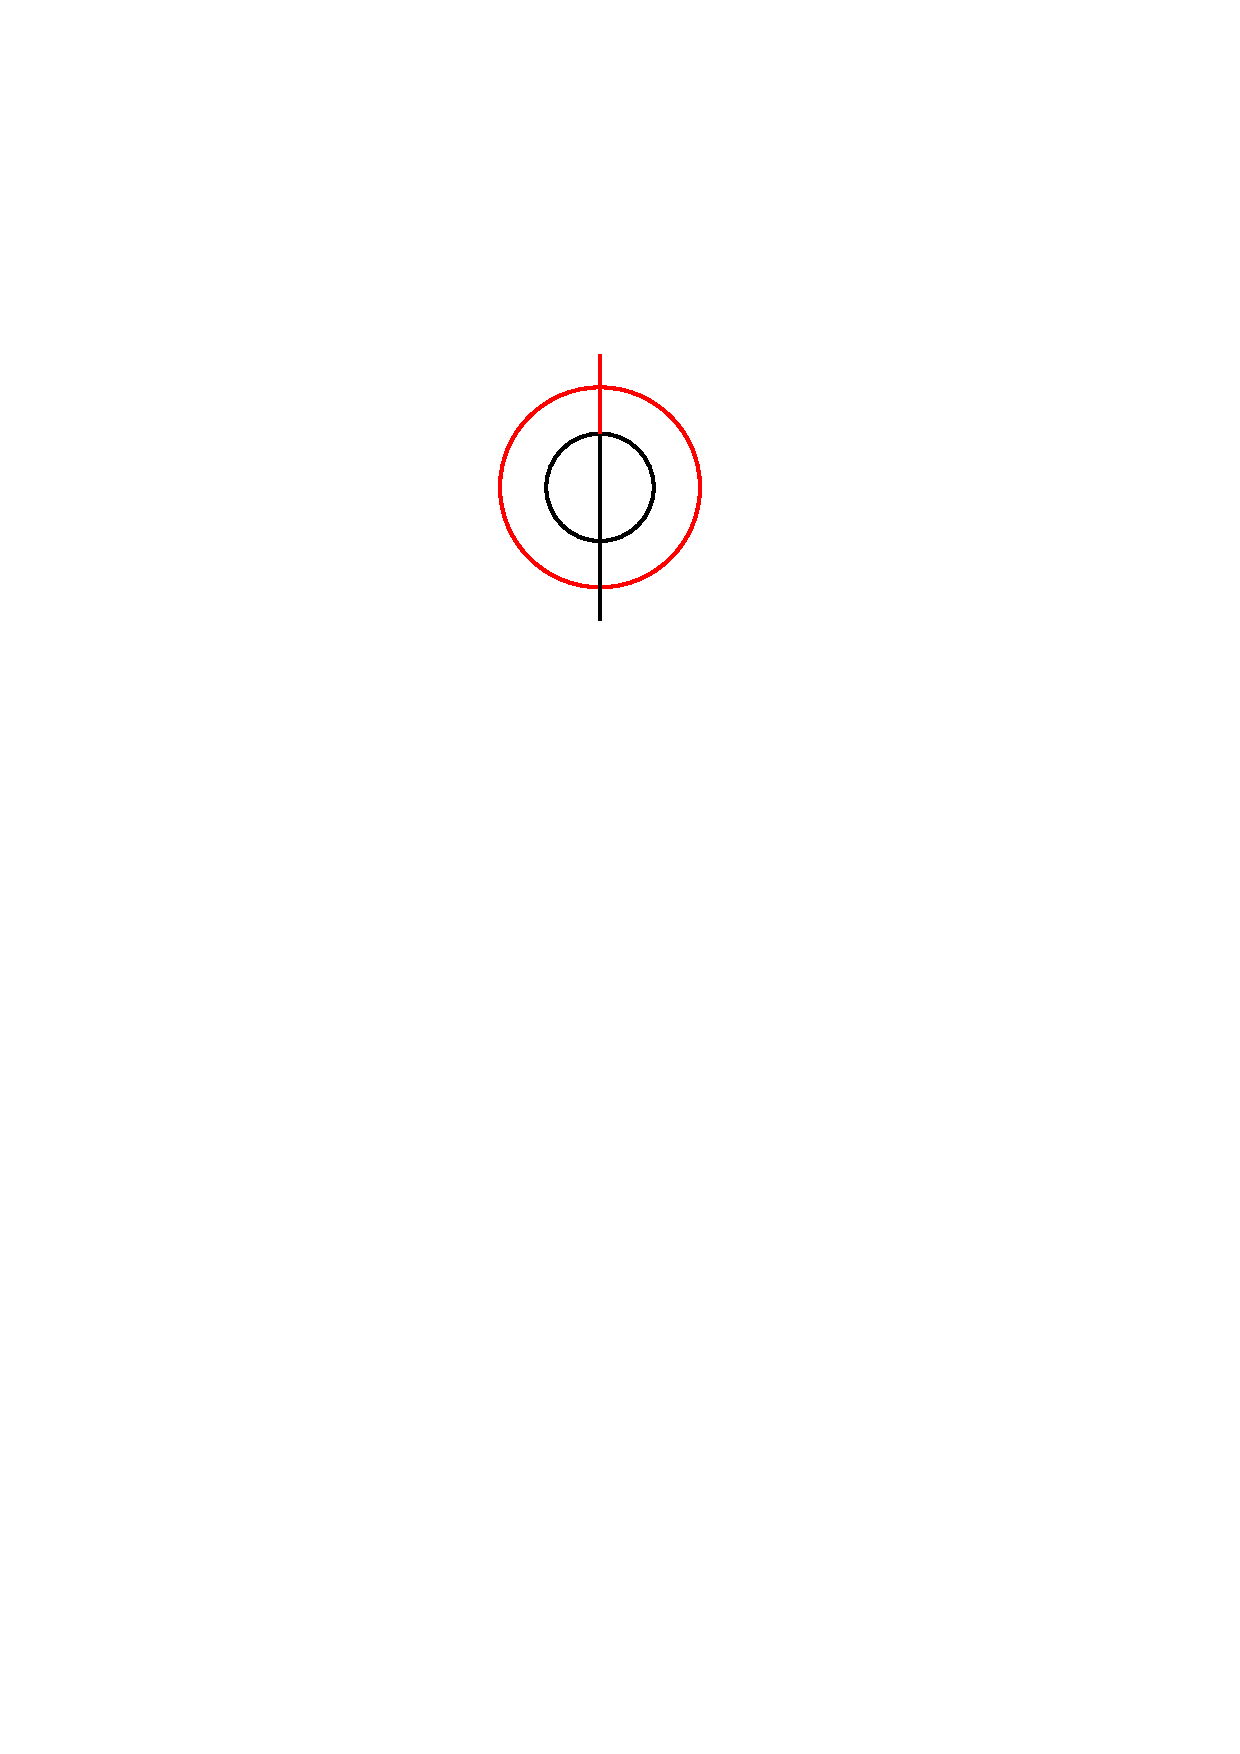
\includegraphics[width=0.25\linewidth]{sauron_s_eye/eye_pt3}
		\hspace{.05\linewidth}\\\vspace{1cm}
		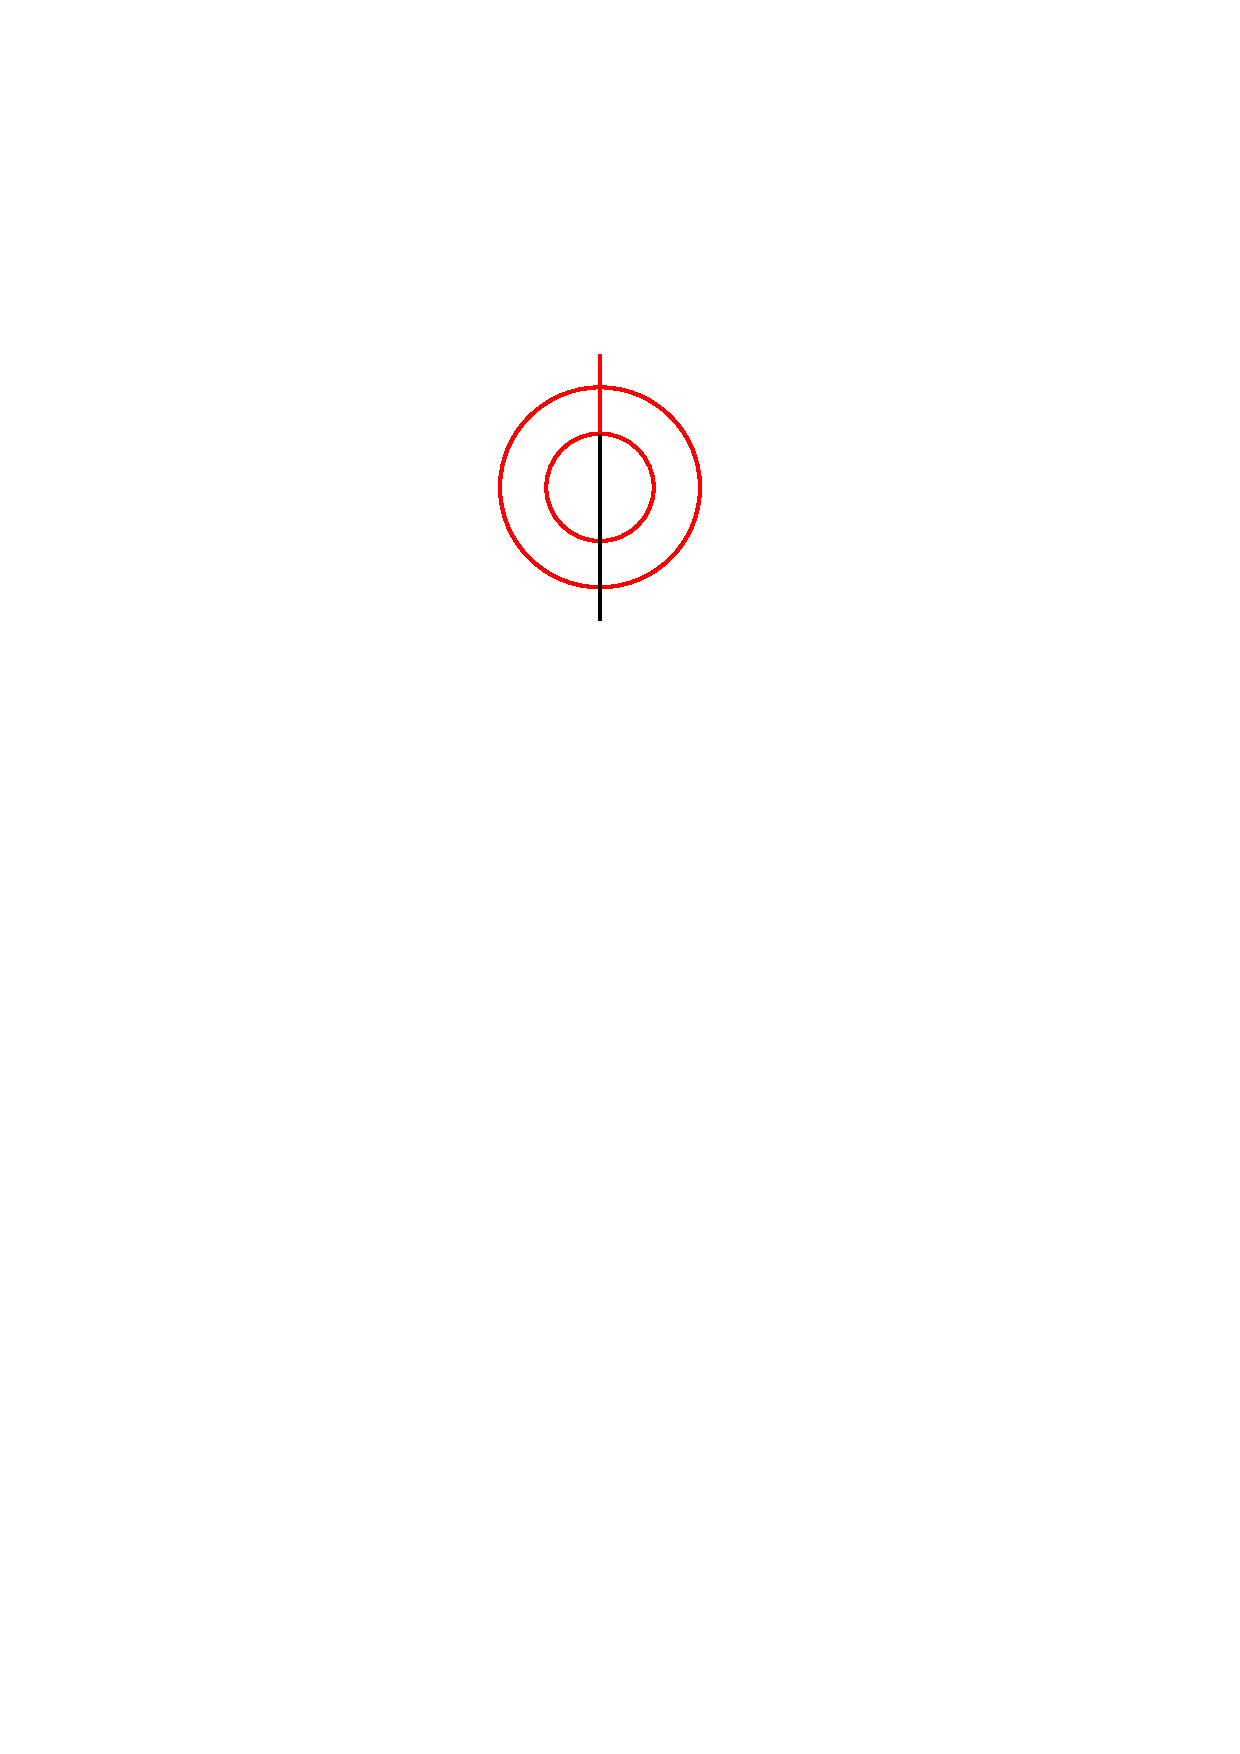
\includegraphics[width=0.25\linewidth]{sauron_s_eye/eye_pt4}
		\hspace{.05\linewidth}
		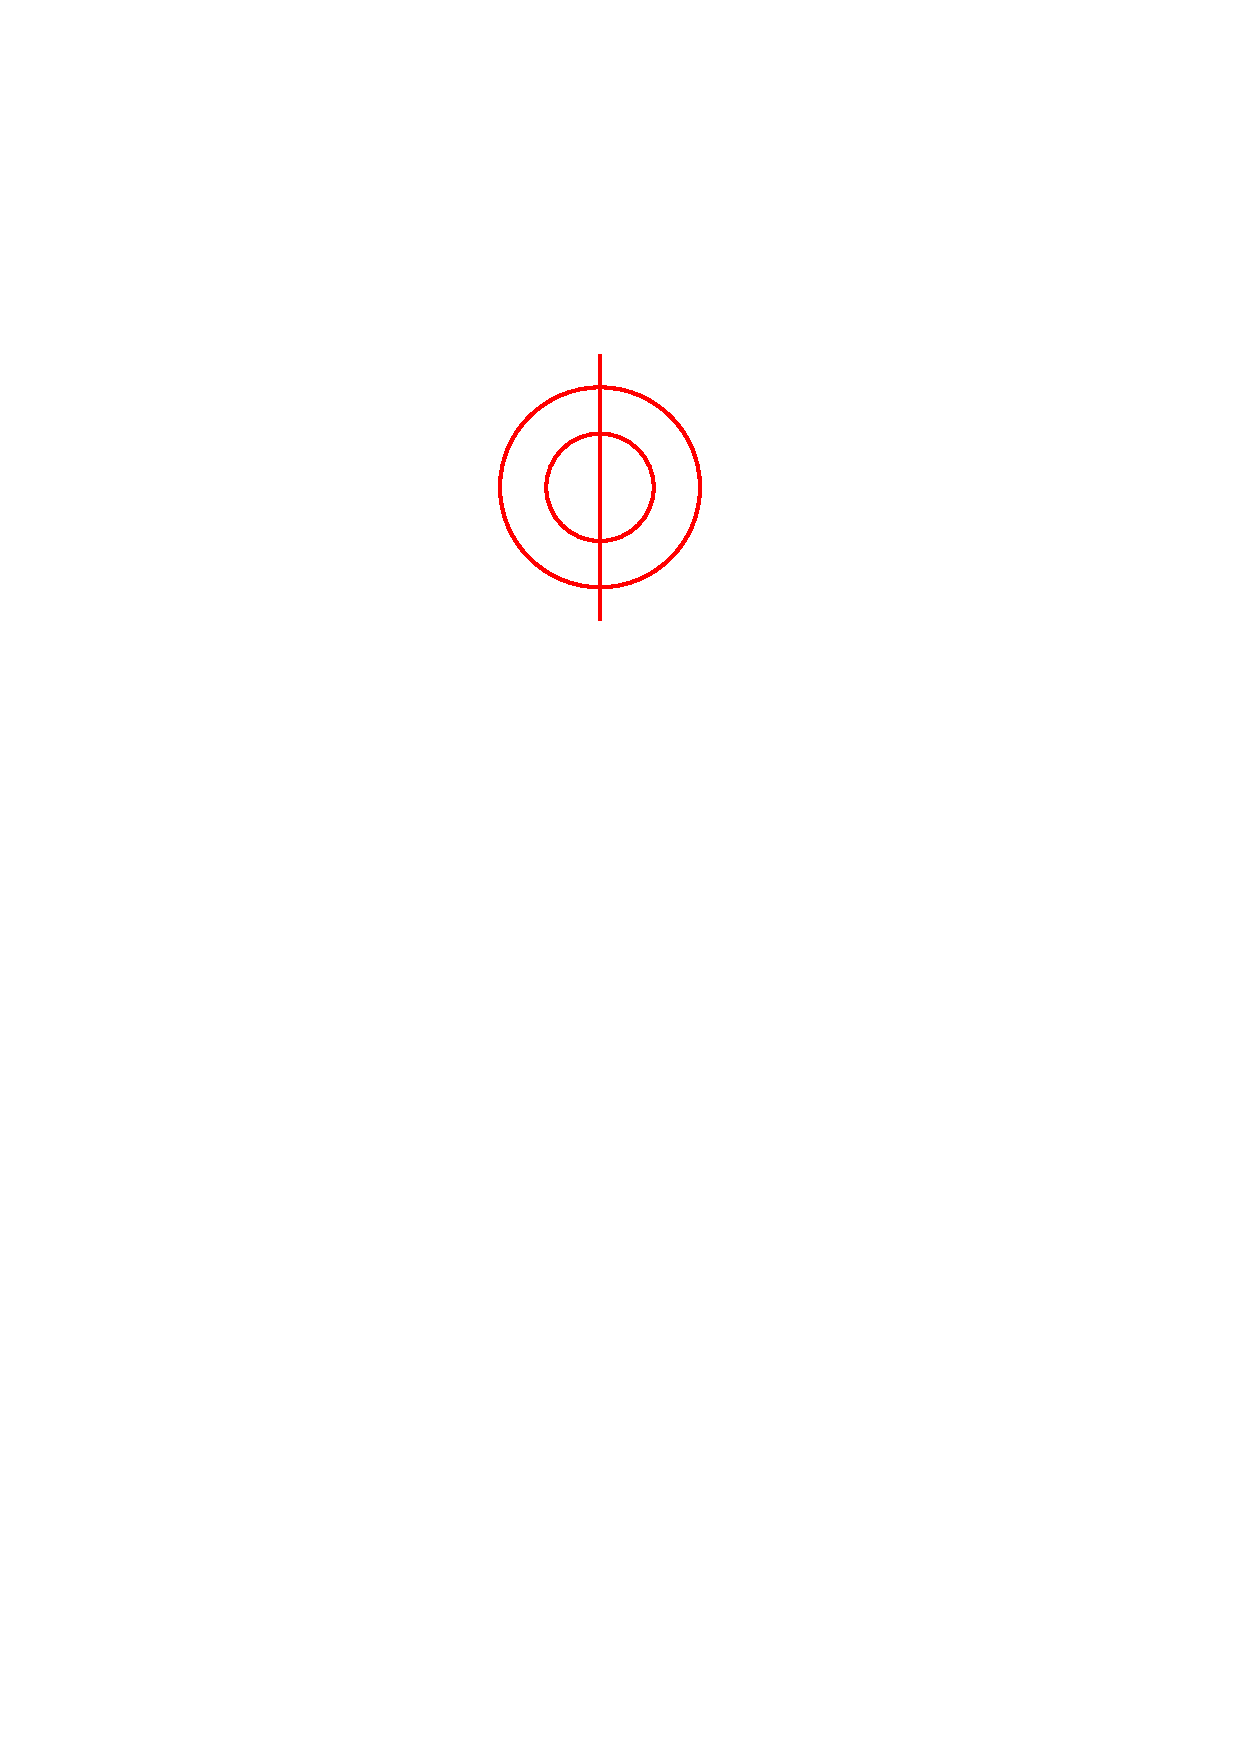
\includegraphics[width=0.25\linewidth]{sauron_s_eye/eye_pt5}
		\hspace{.05\linewidth}
		\label{fig:eyept1}
	\end{figure}
	\section{O Barco}
	
	O barco apresentou o mesmo problema do Wolverine pois para todo o contorno escolhido um linha sempre ficava ``para trás'' sendo impossível de percorrê-la sem passar num contorno já utilizado.
	\newpage
	\section{A Casa}
	\vspace{-.5cm}
	\begin{figure}[H]
		\centering
		
\includegraphics[width=0.3\linewidth]{house/house}
		\label{fig:house}
	\end{figure}
	\begin{figure}[H]
		\centering
		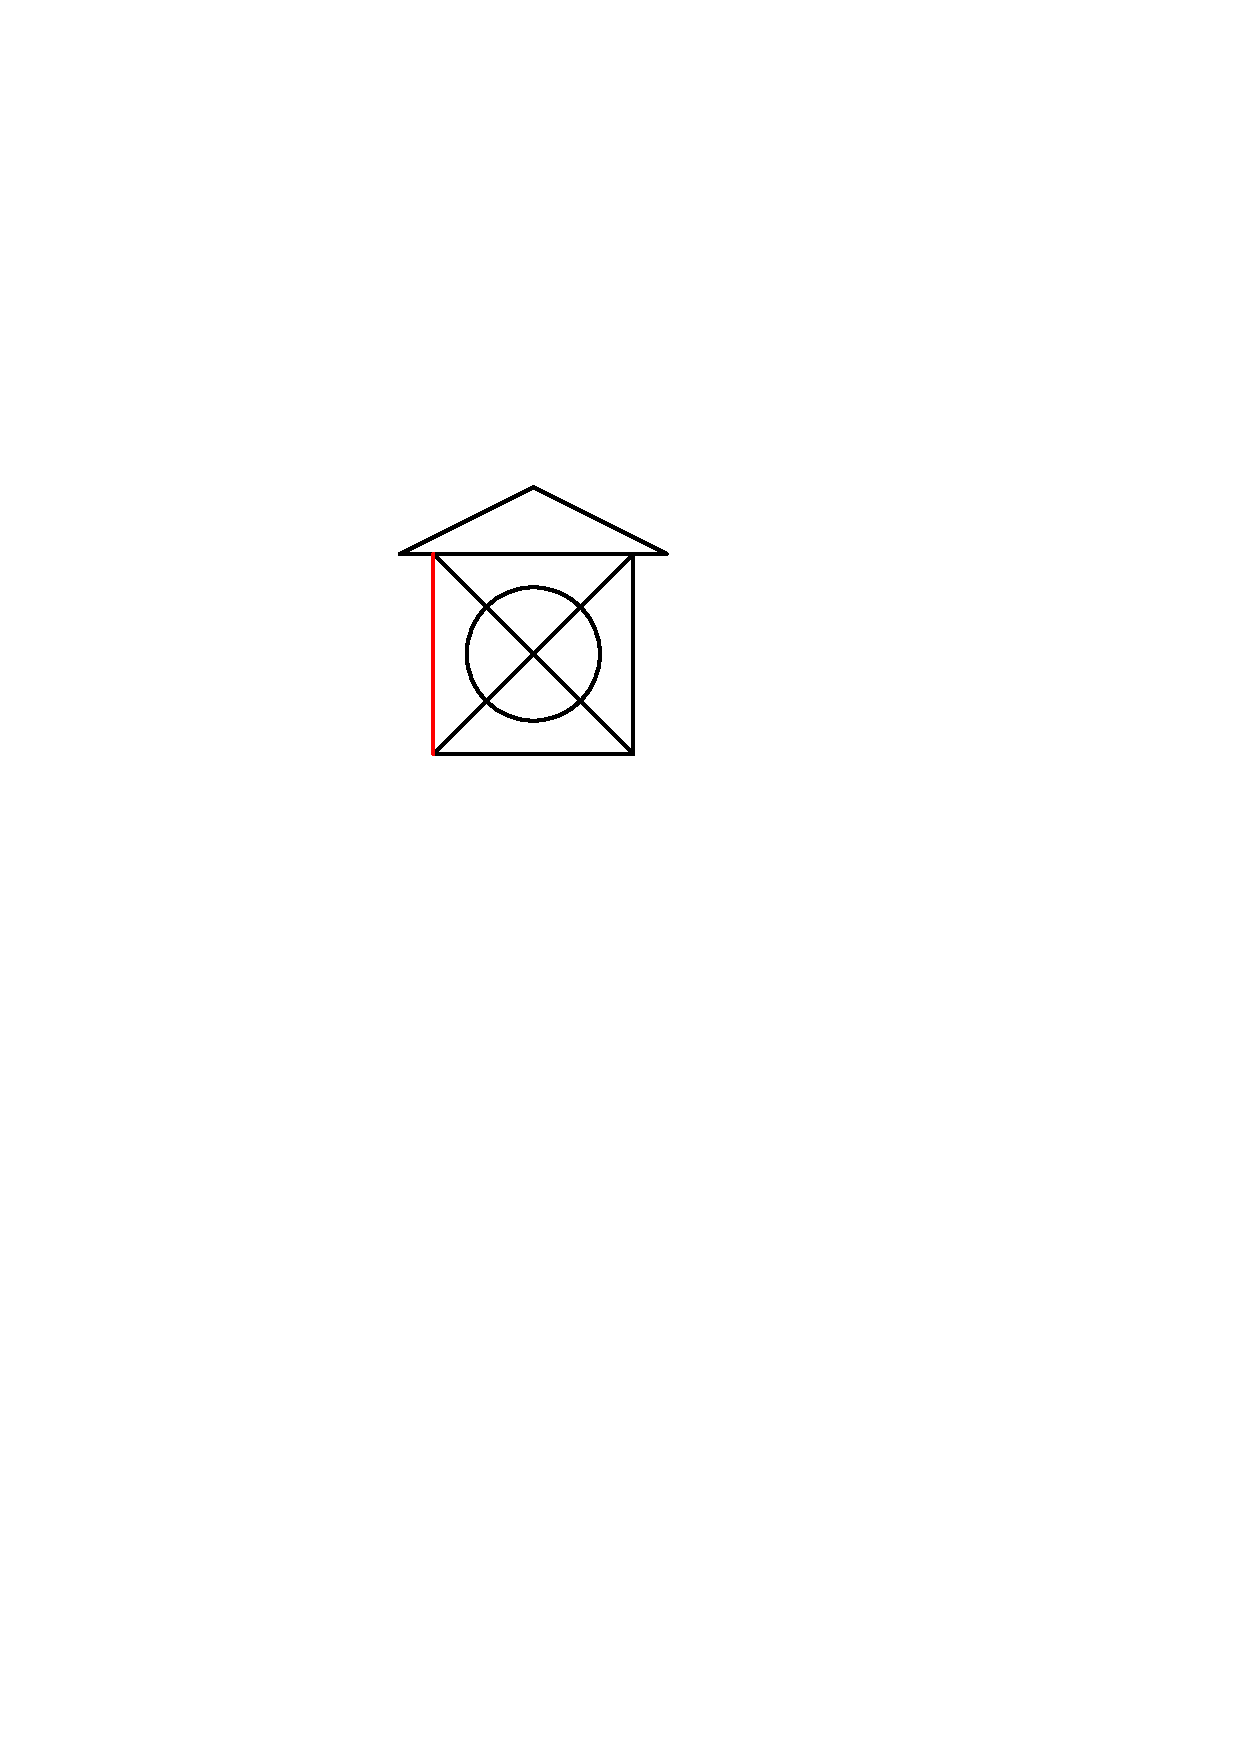
\includegraphics[width=0.25\linewidth]{house/house_pt1}
		\hspace{.05\linewidth}
		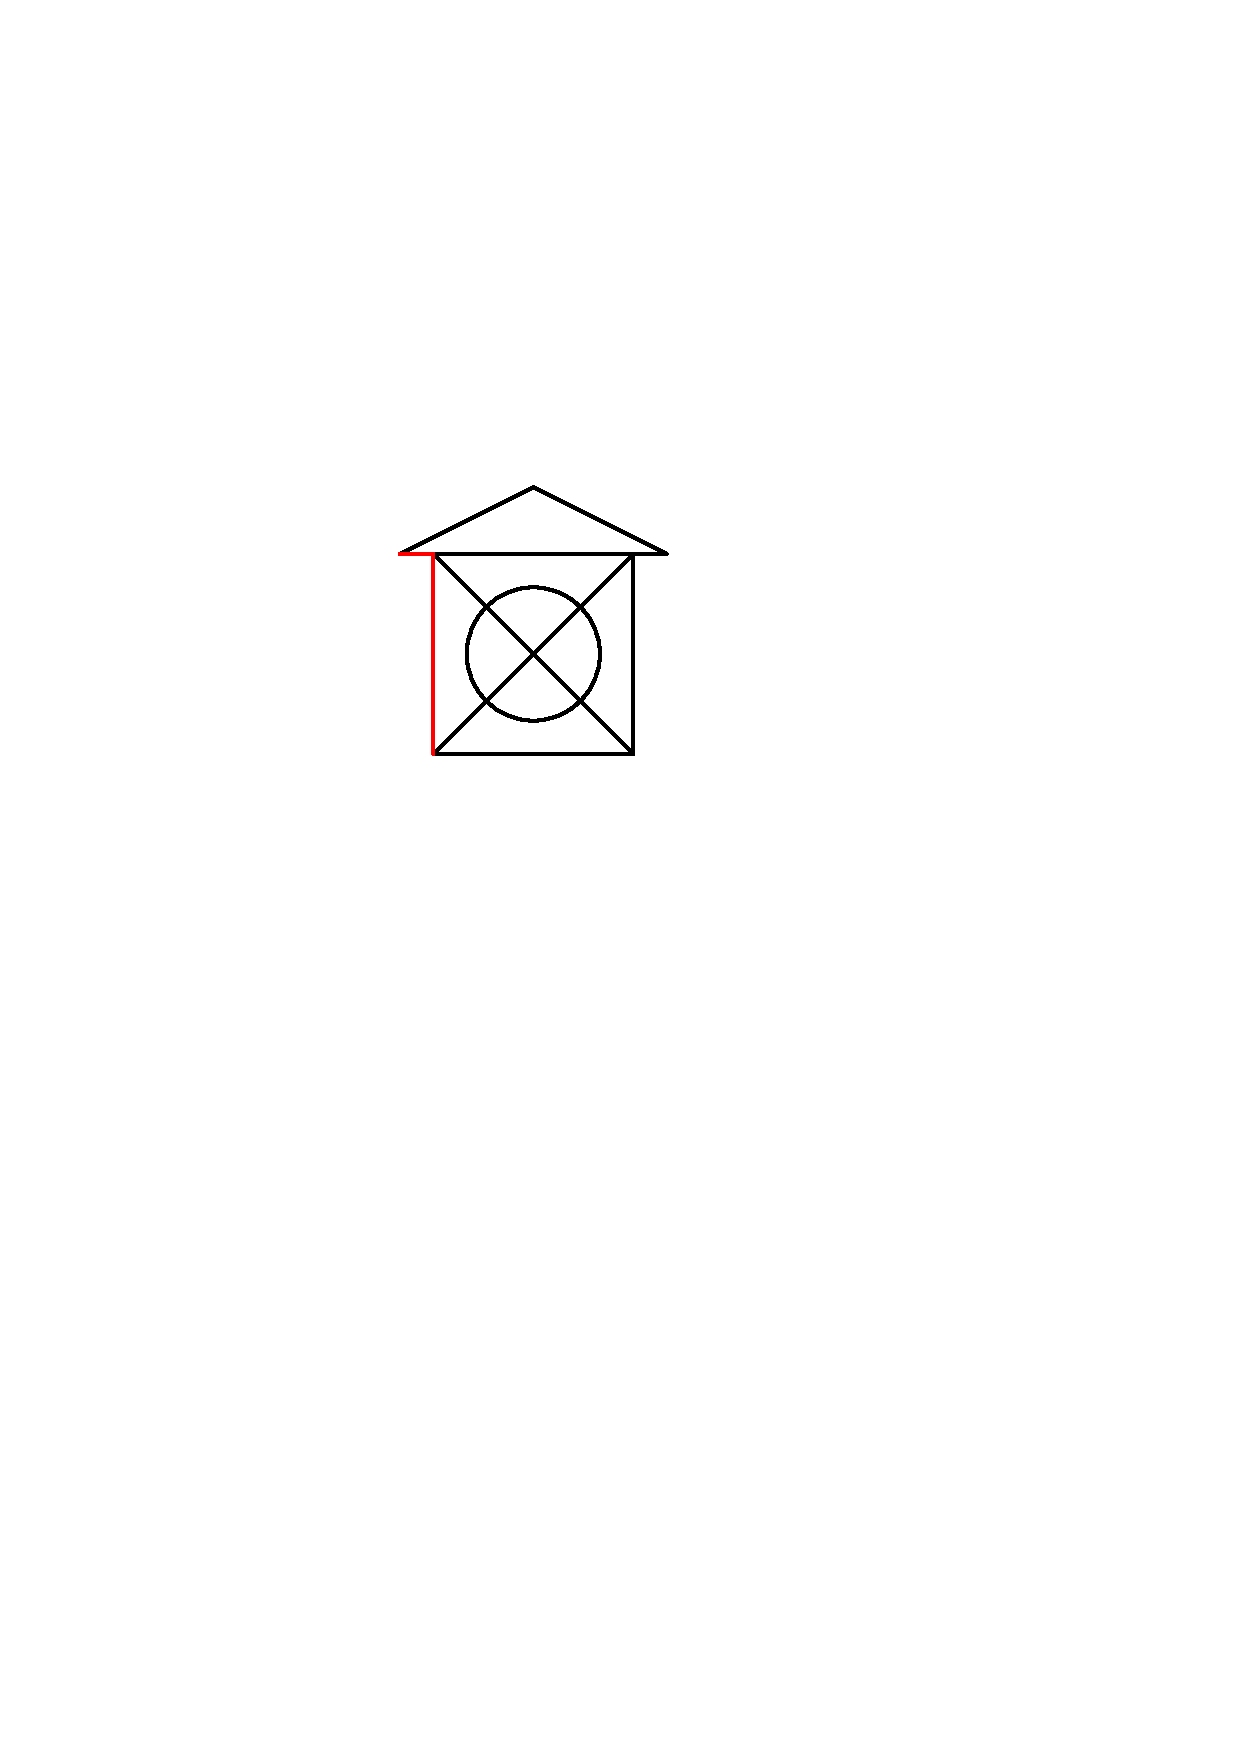
\includegraphics[width=0.25\linewidth]{house/house_pt2}
		\hspace{.05\linewidth}
		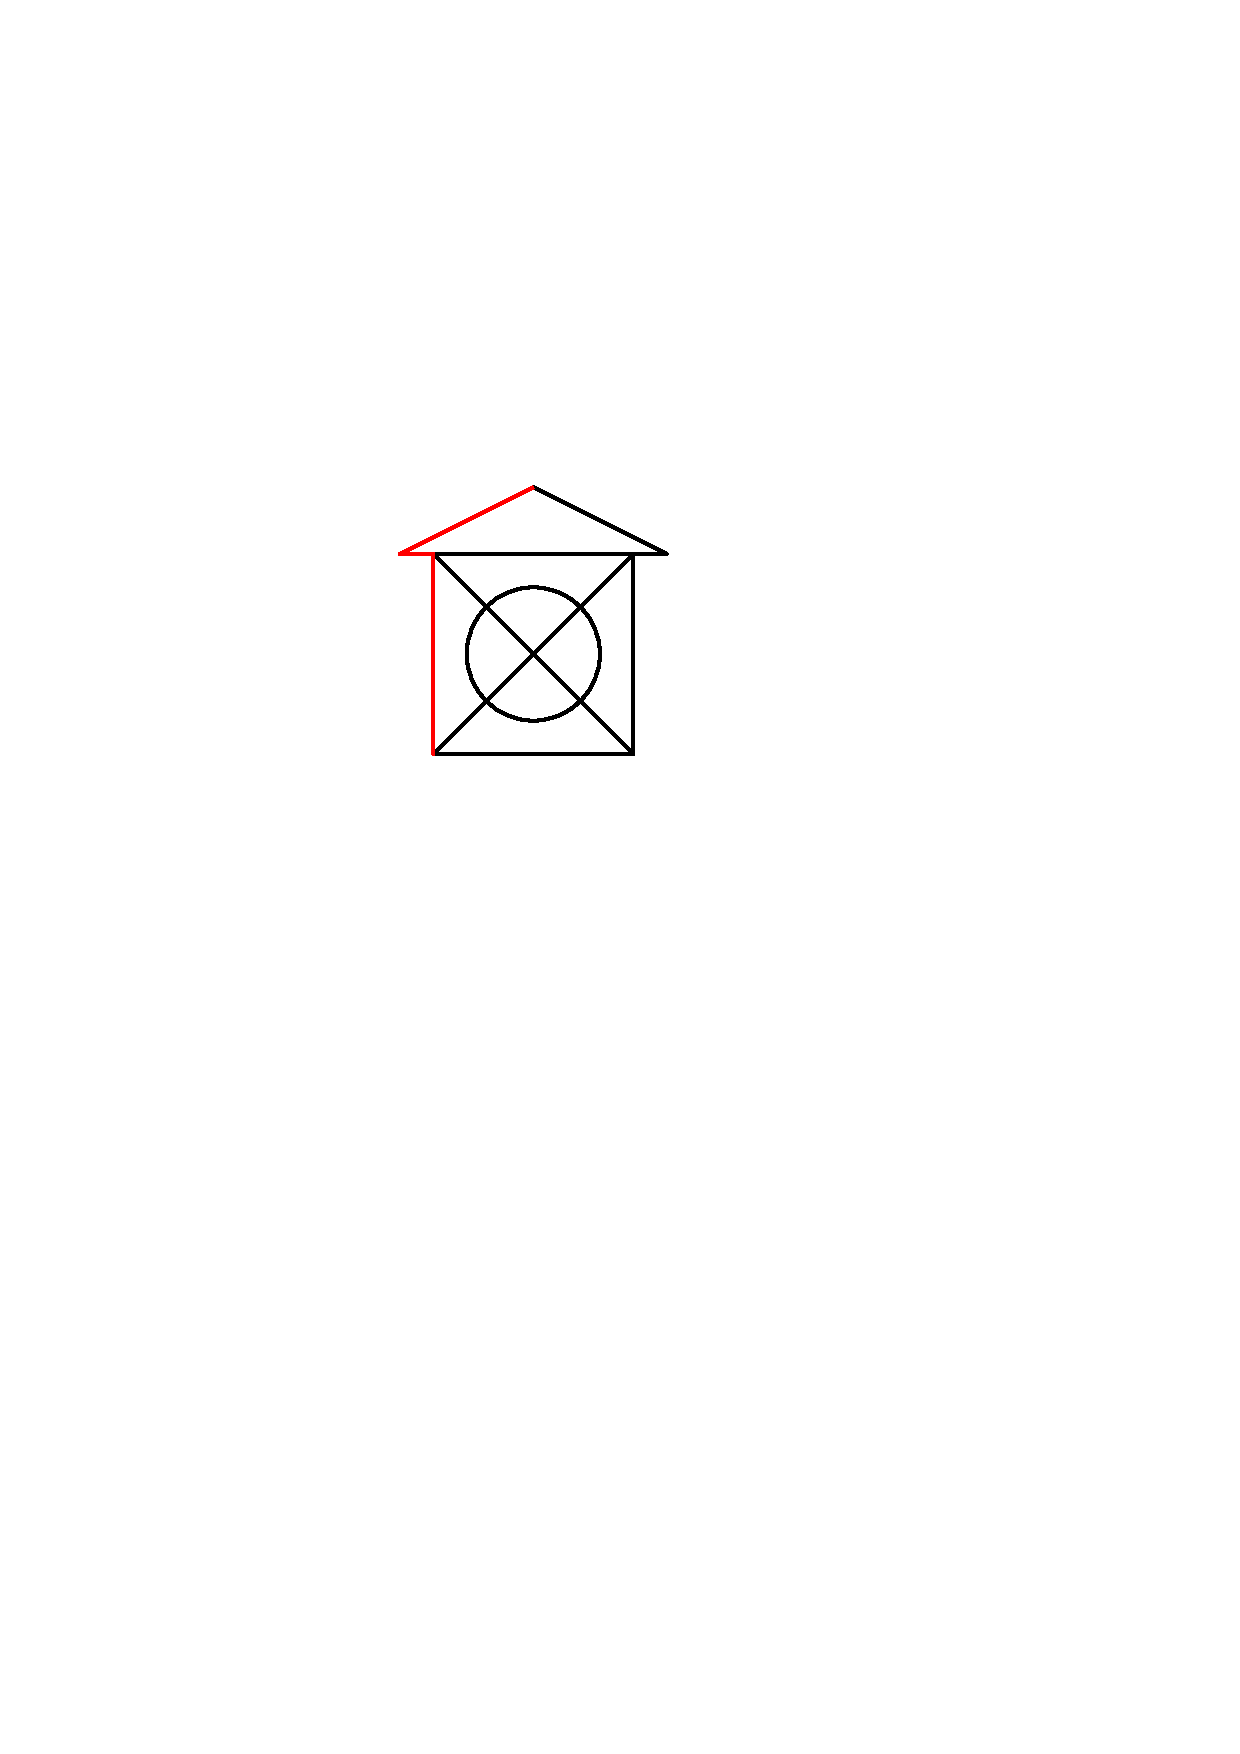
\includegraphics[width=0.25\linewidth]{house/house_pt3}
		\hspace{.05\linewidth}\\\vspace{1cm}
		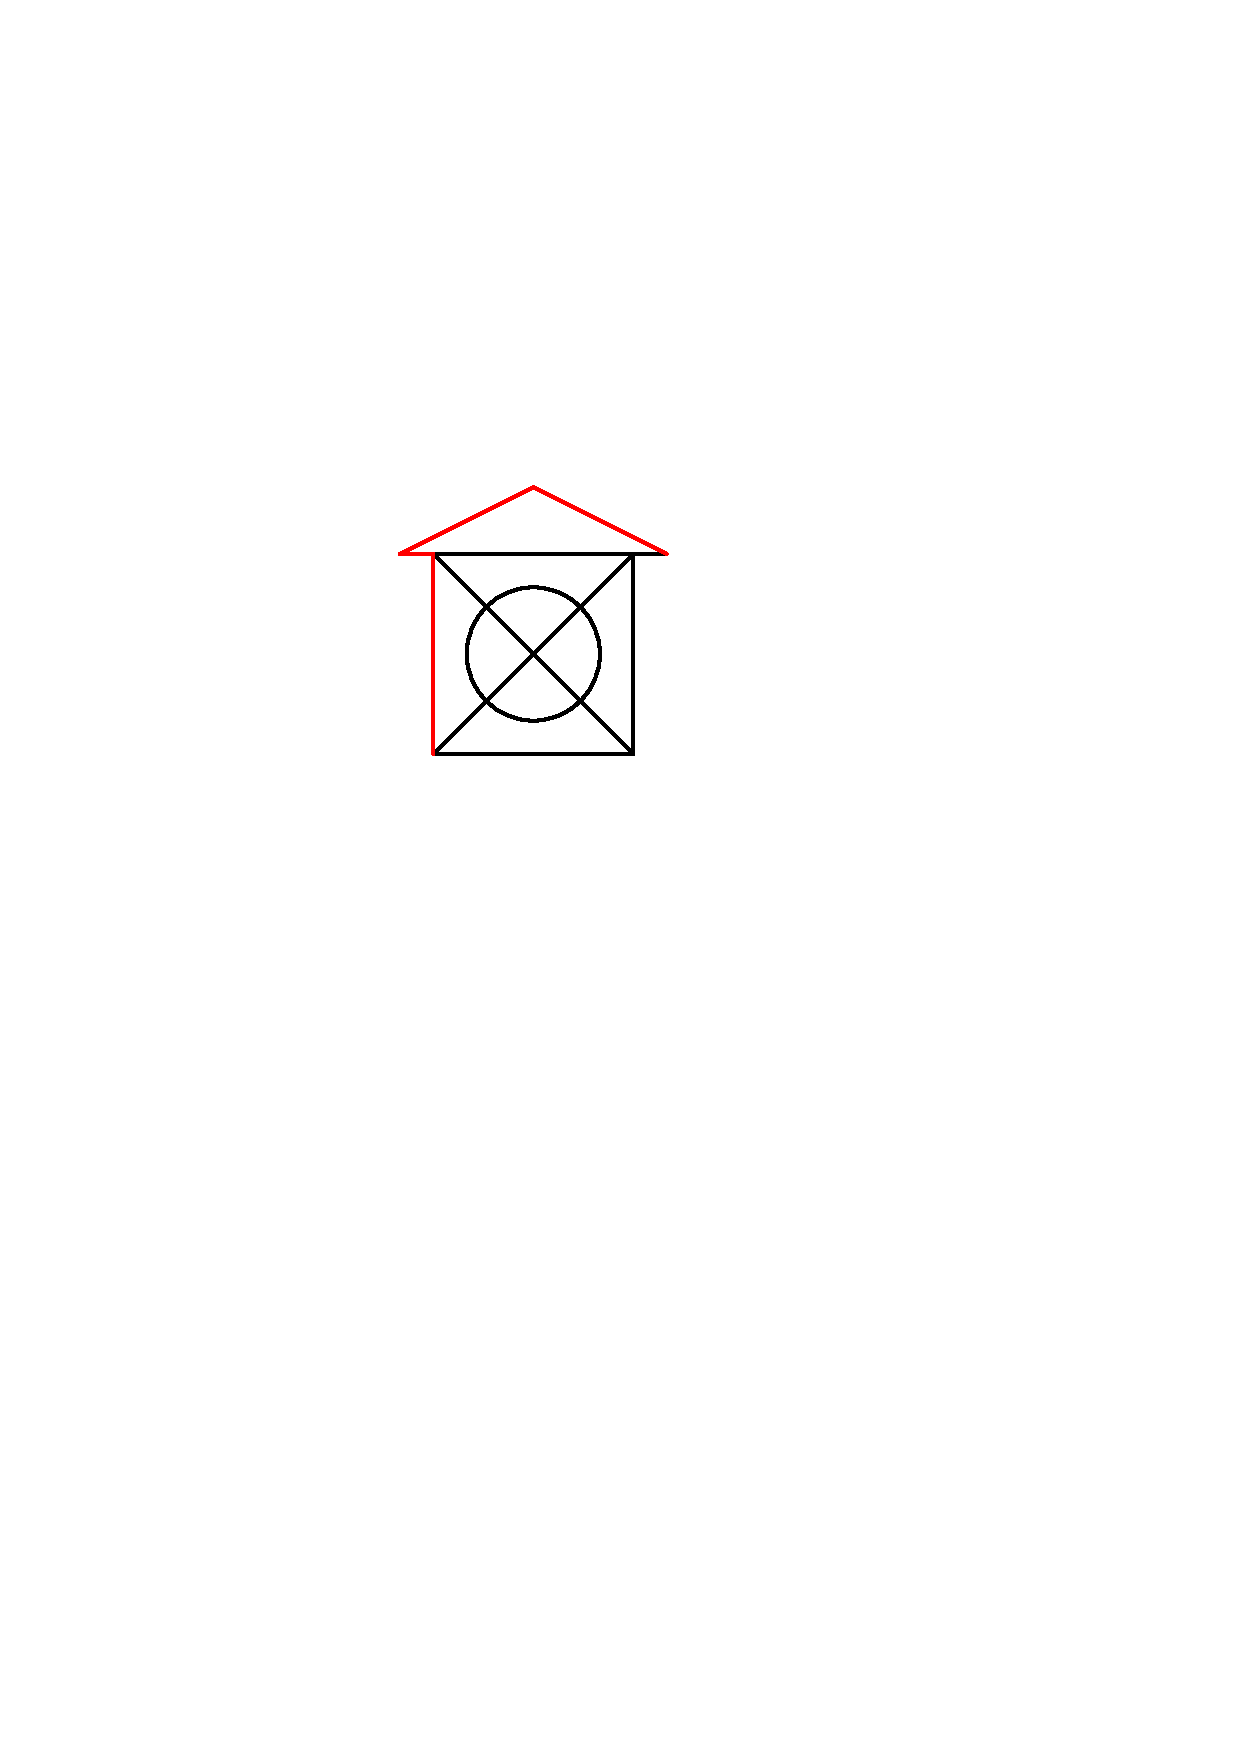
\includegraphics[width=0.25\linewidth]{house/house_pt4}
		\hspace{.05\linewidth}
		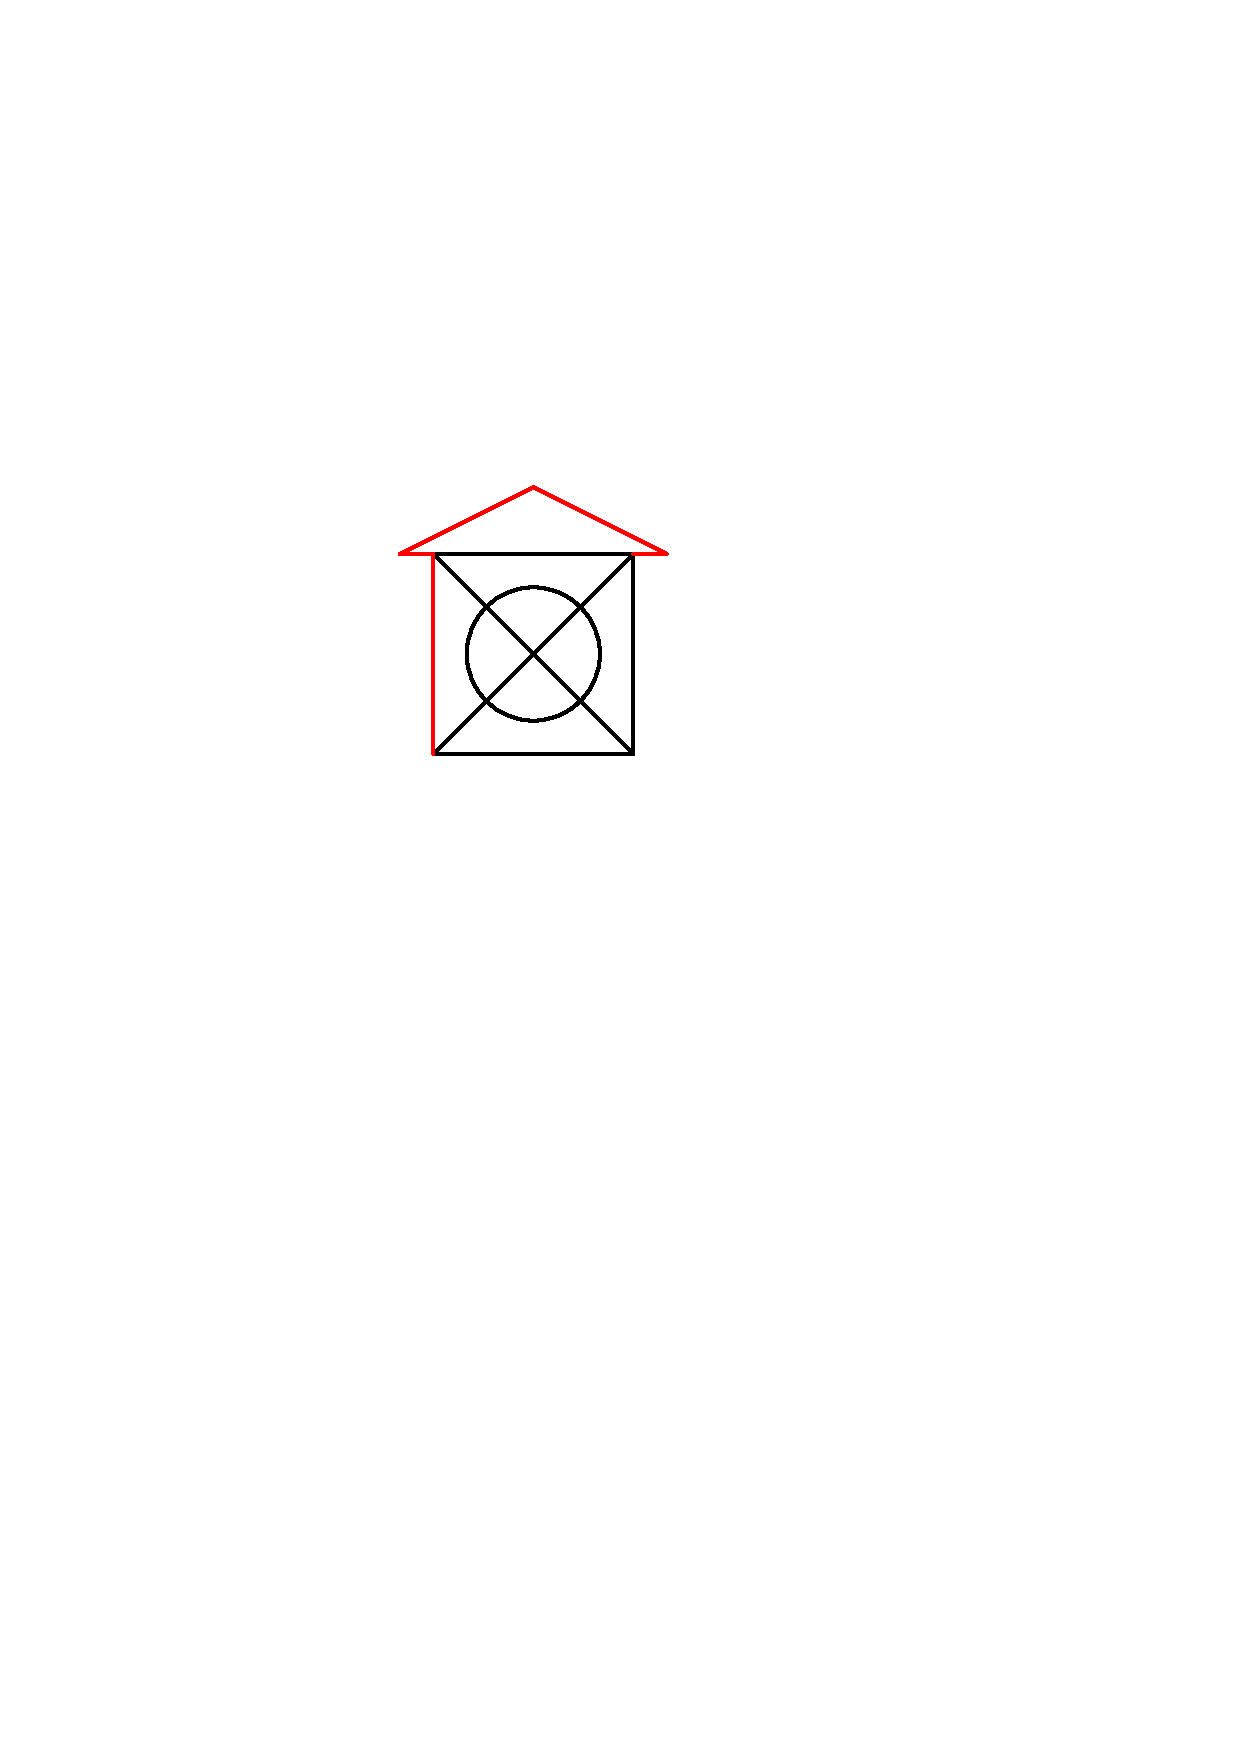
\includegraphics[width=0.25\linewidth]{house/house_pt5}
		\hspace{.05\linewidth}
		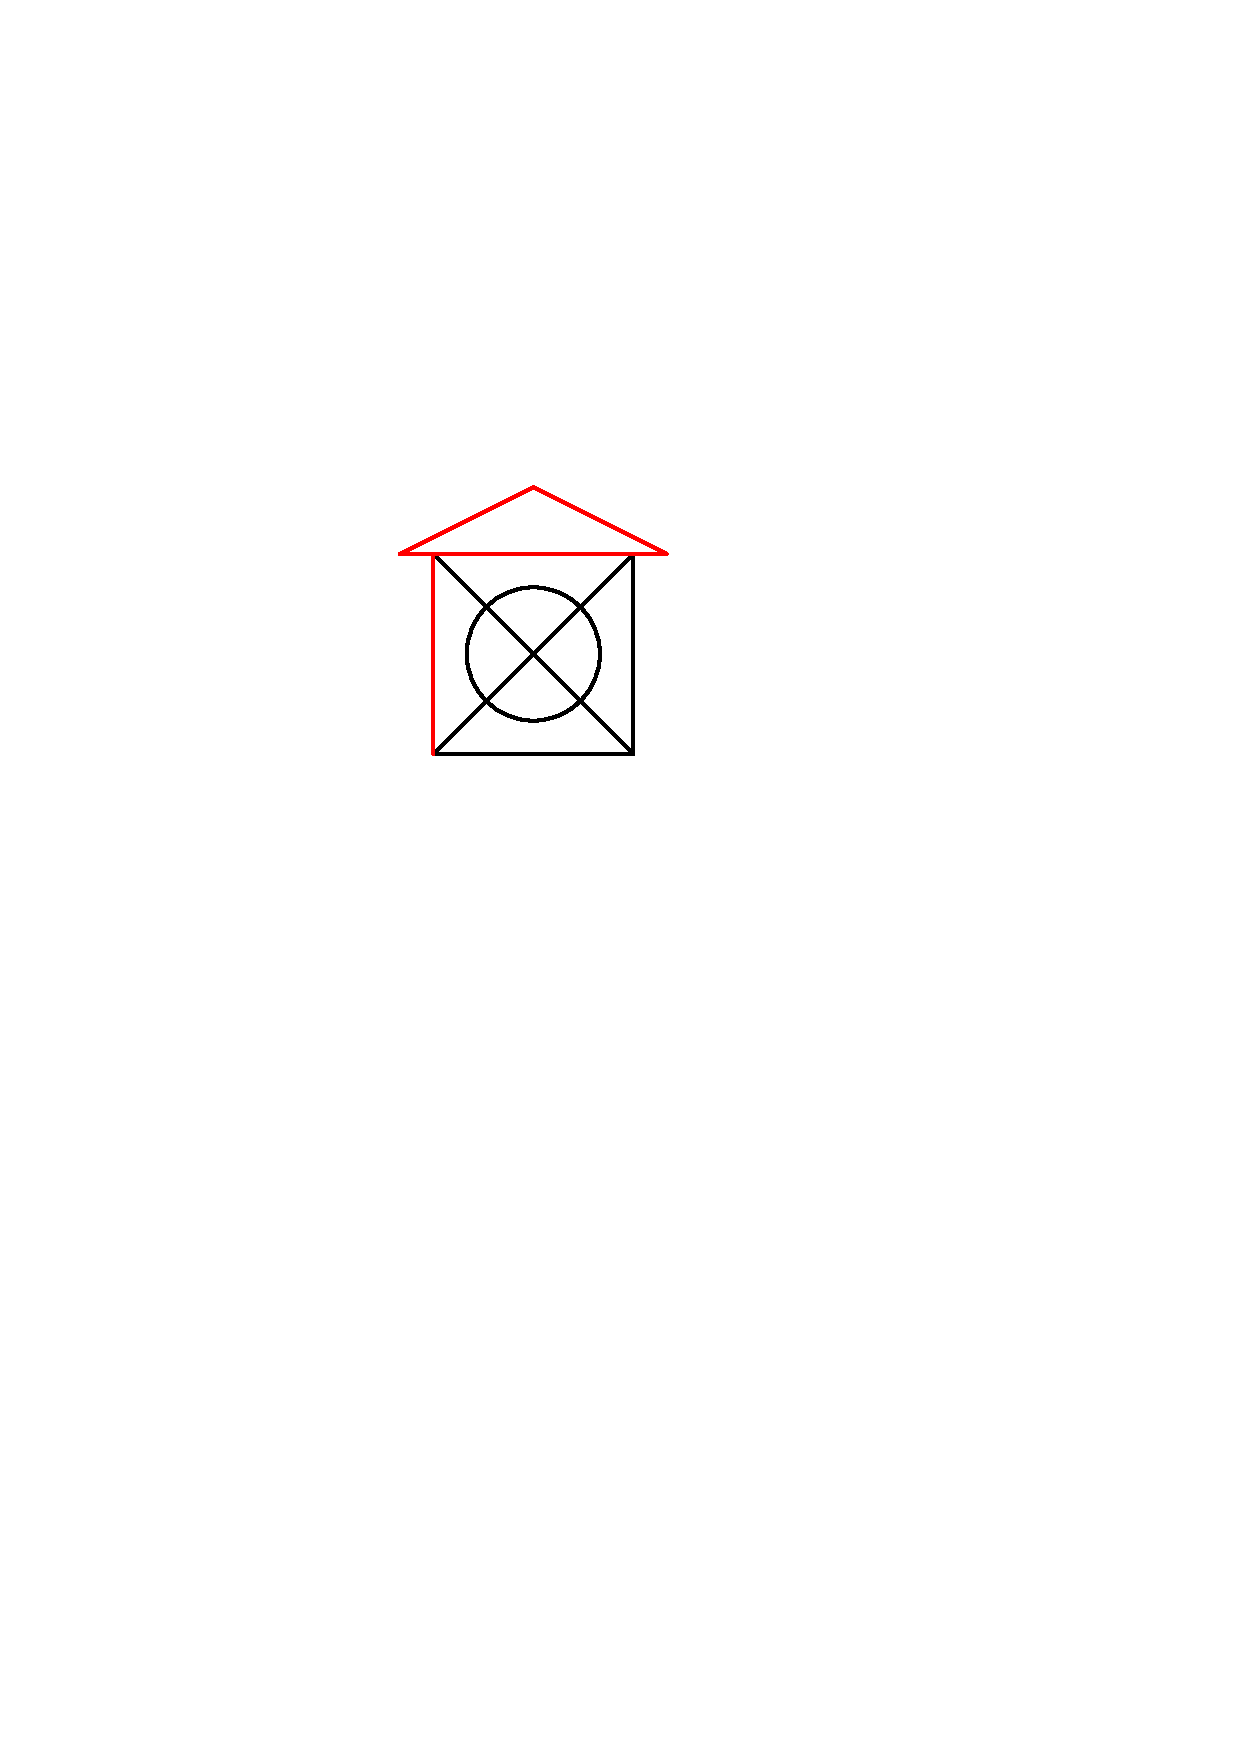
\includegraphics[width=0.25\linewidth]{house/house_pt6}
		\hspace{.05\linewidth}\\\vspace{1cm}
		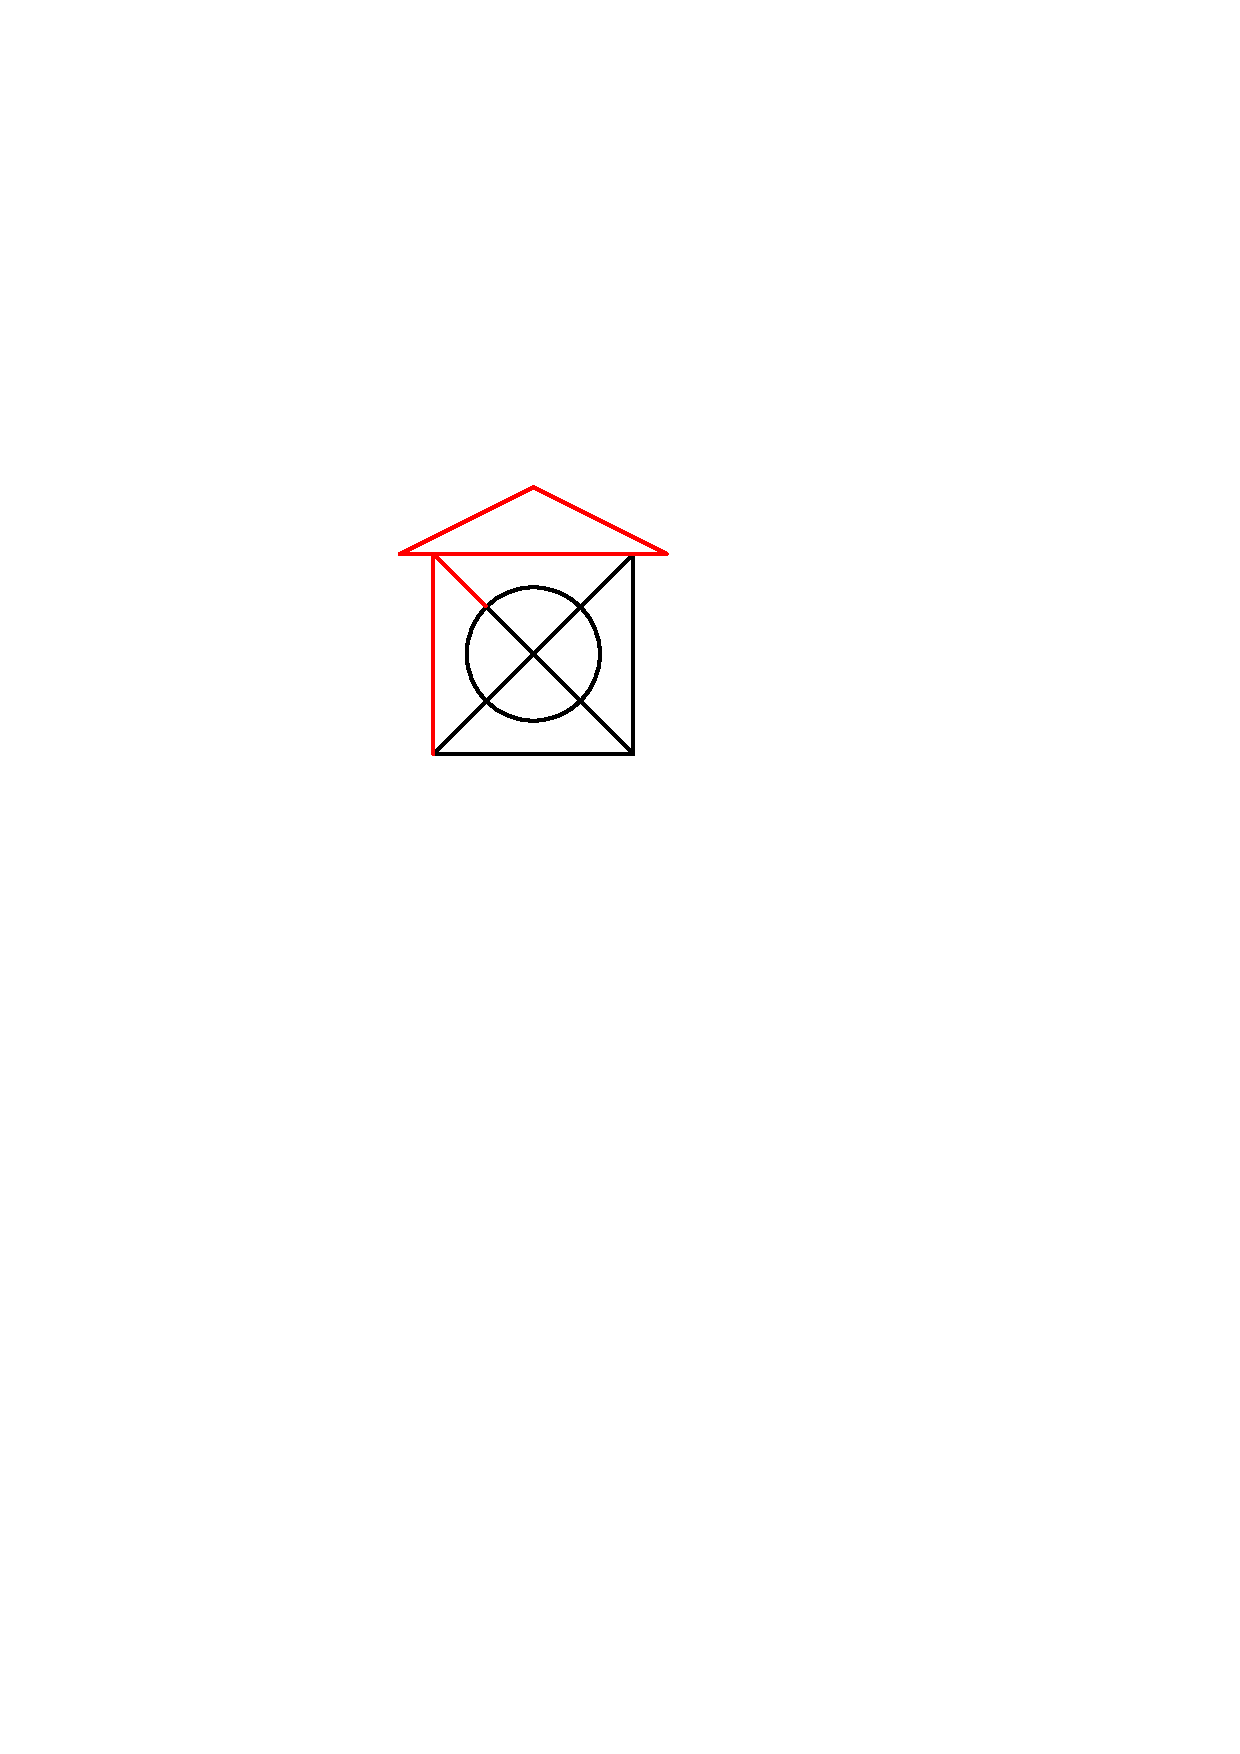
\includegraphics[width=0.25\linewidth]{house/house_pt7}
		\hspace{.05\linewidth}
		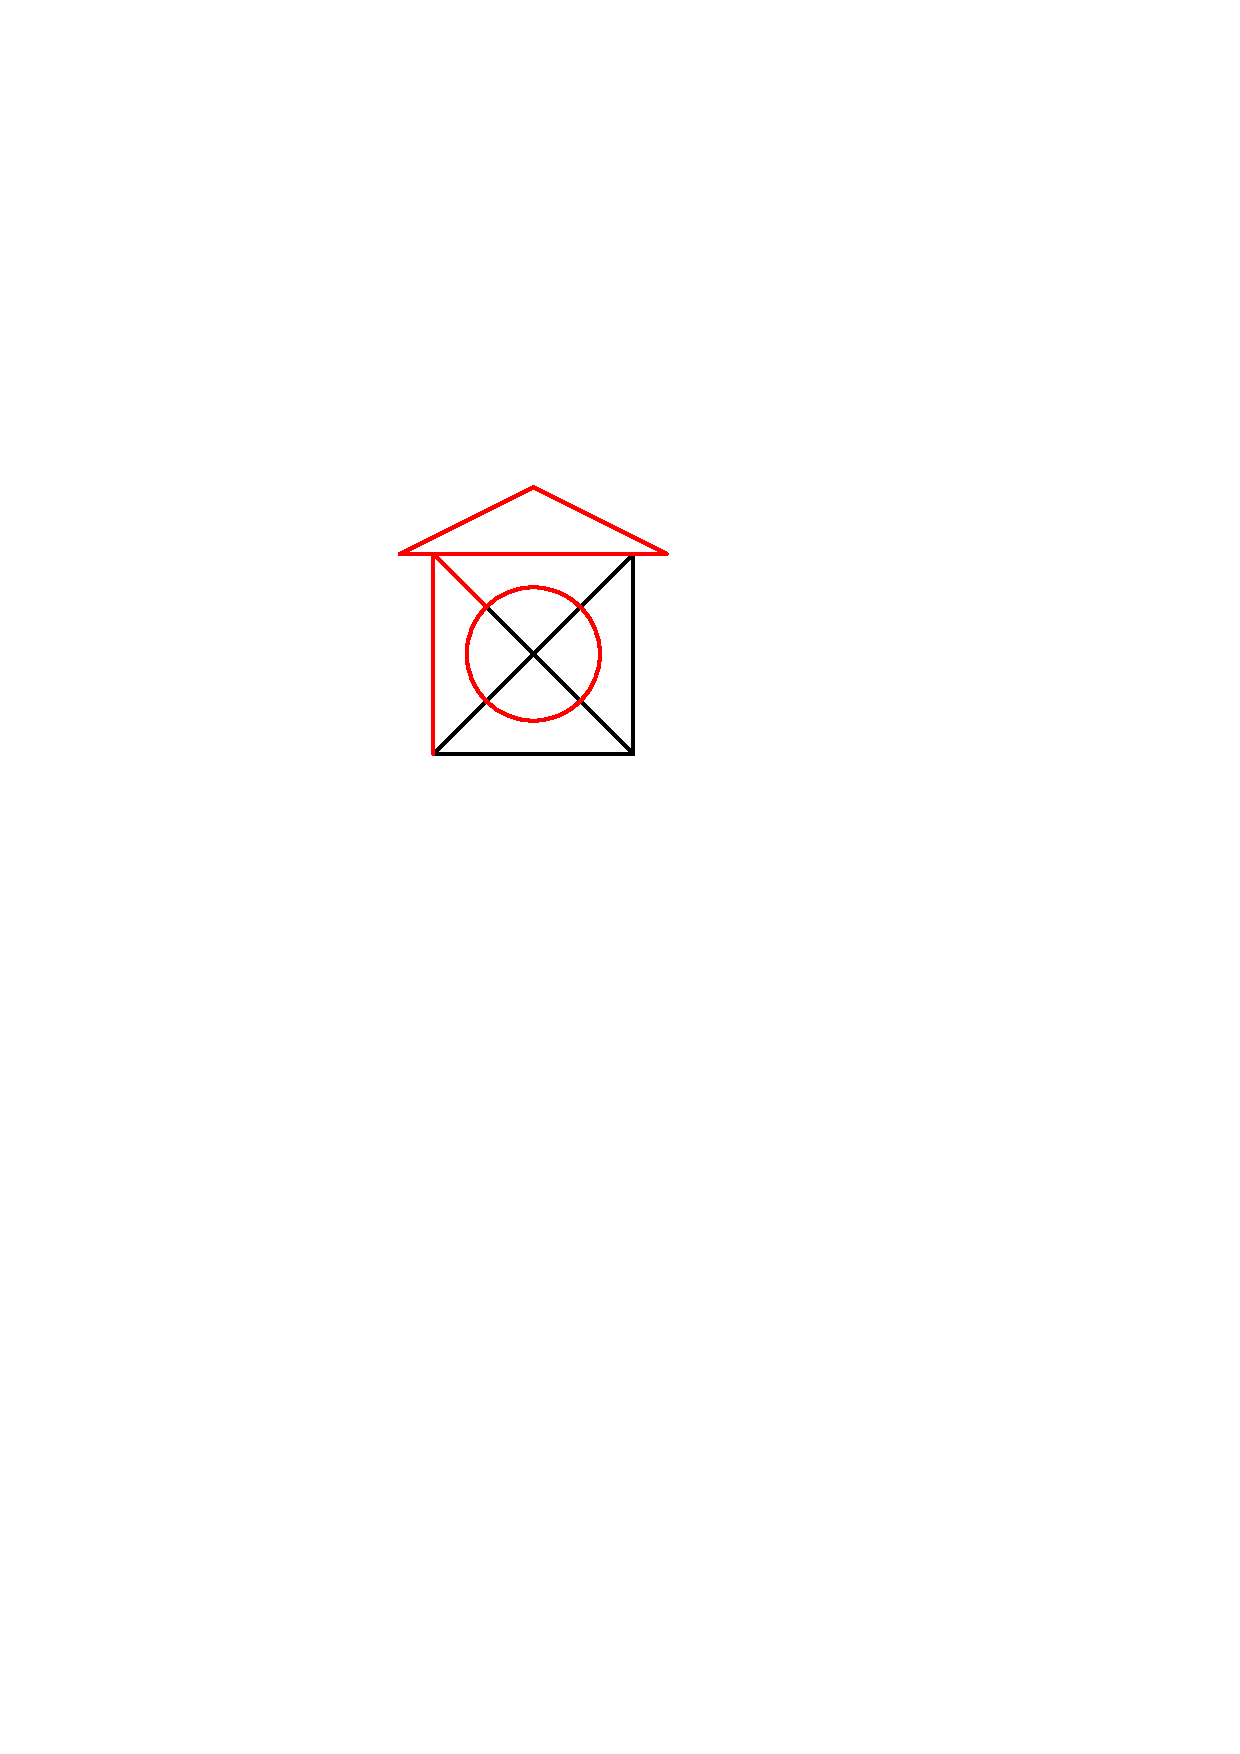
\includegraphics[width=0.25\linewidth]{house/house_pt8}
		\hspace{.05\linewidth}
		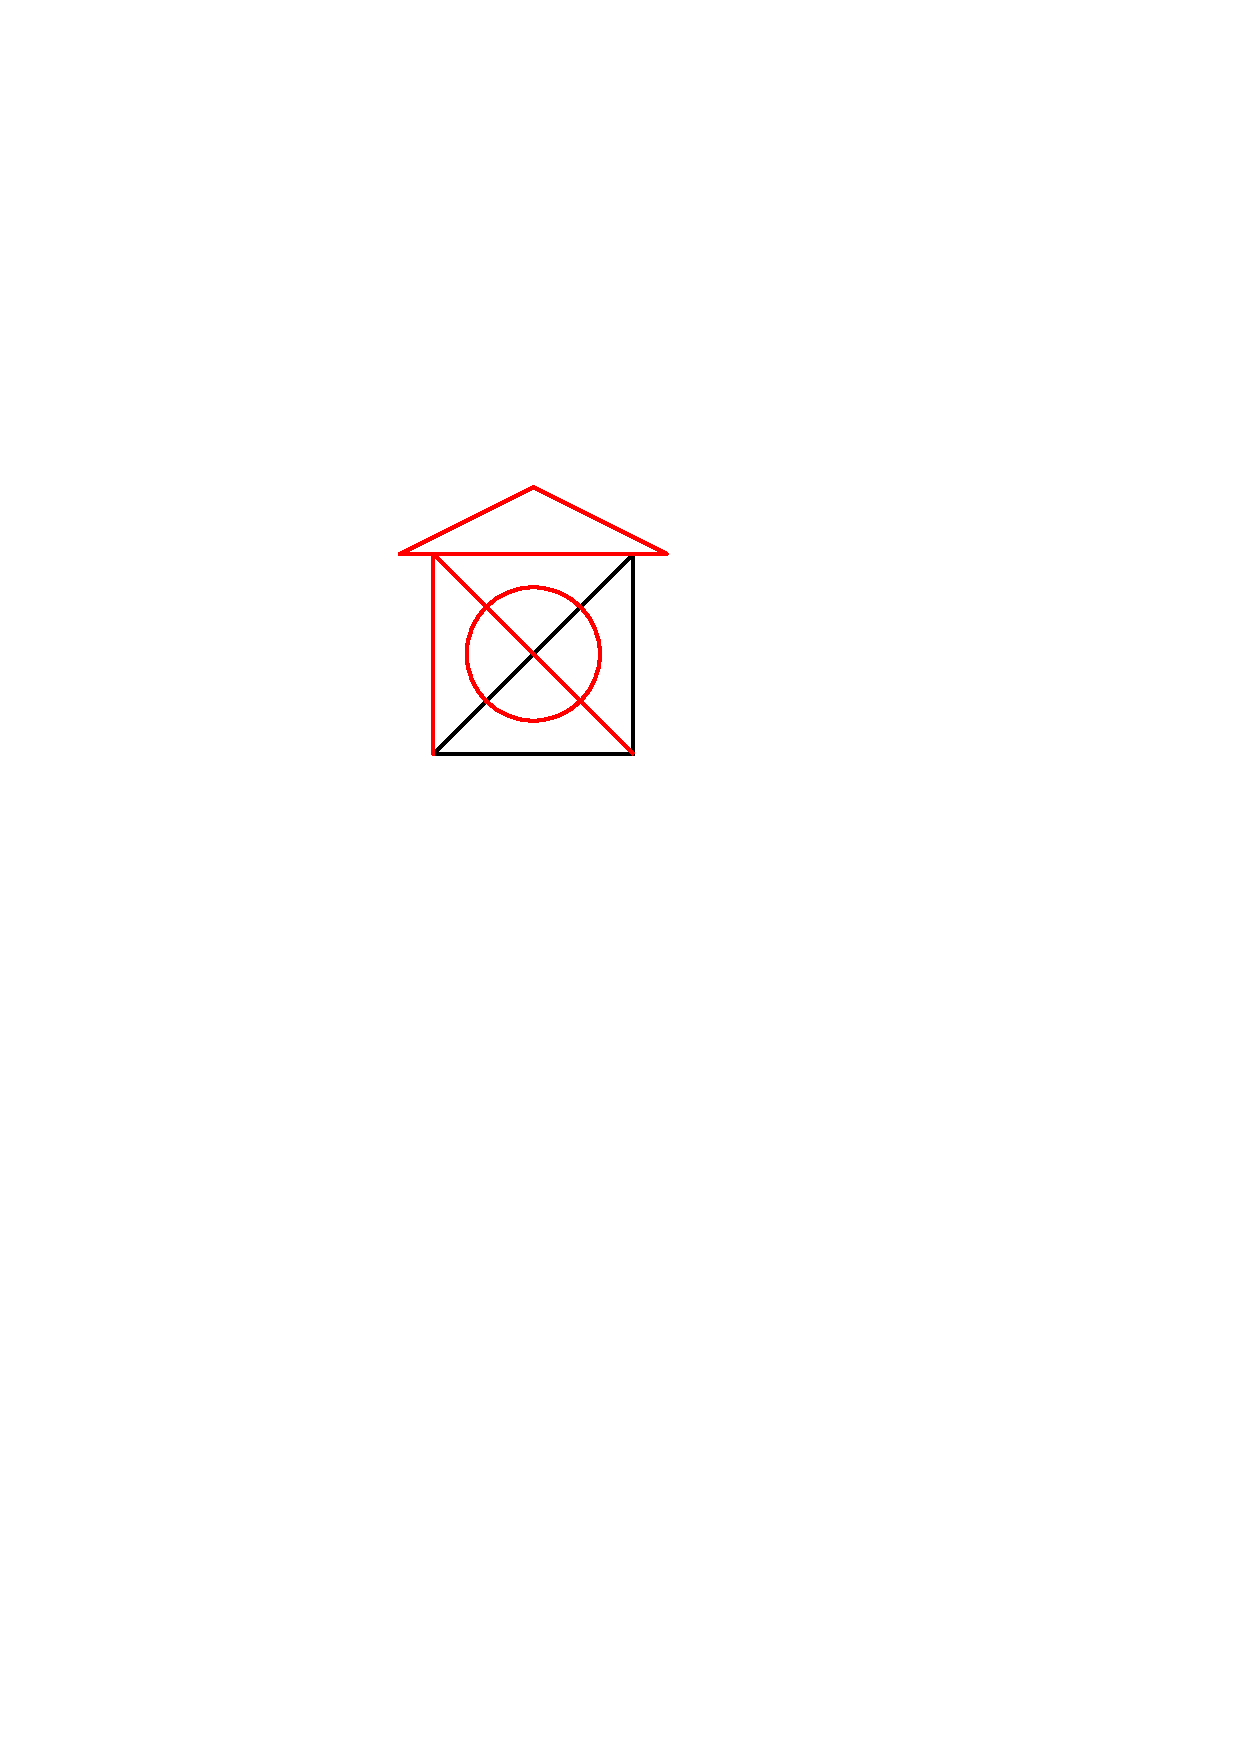
\includegraphics[width=0.25\linewidth]{house/house_pt9}
		\hspace{.05\linewidth}\\\vspace{1cm}
		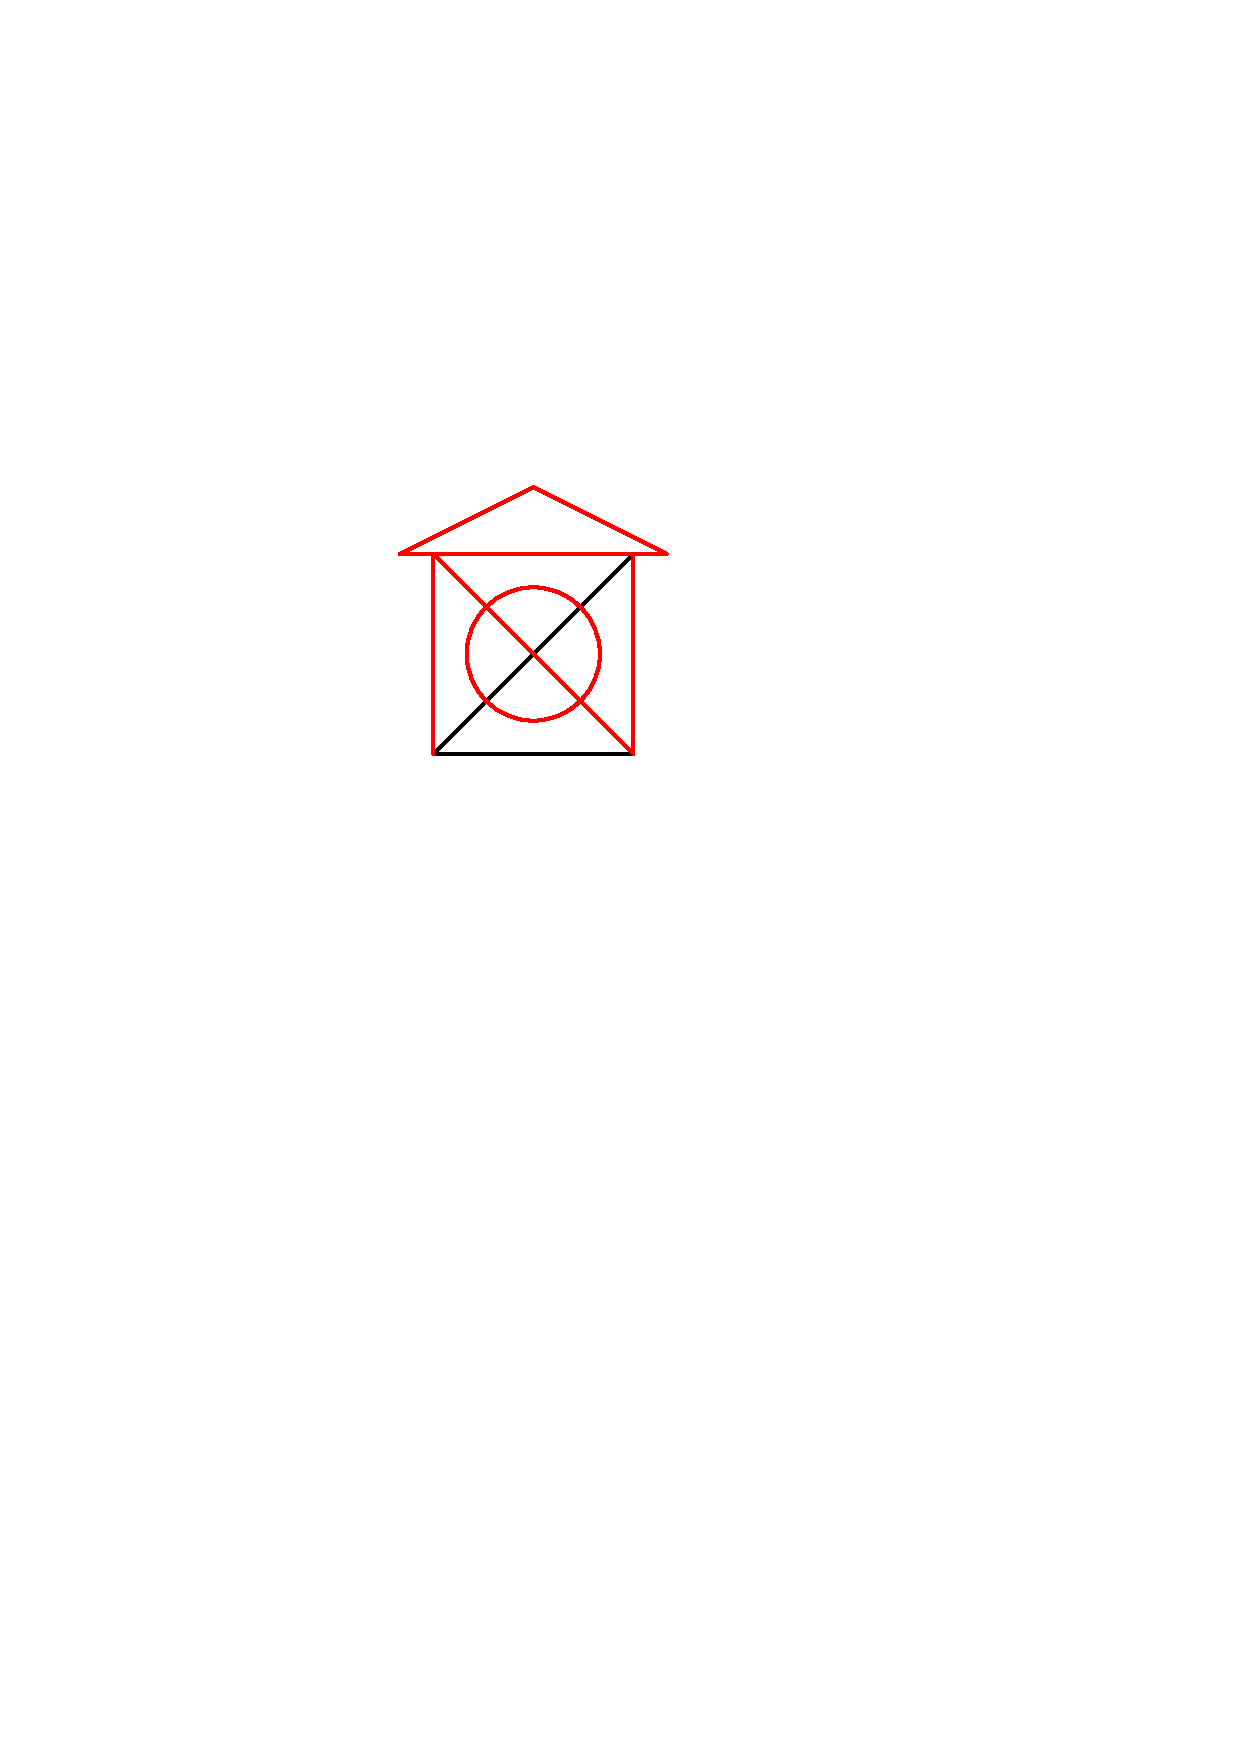
\includegraphics[width=0.25\linewidth]{house/house_pt10}
		\hspace{.05\linewidth}
		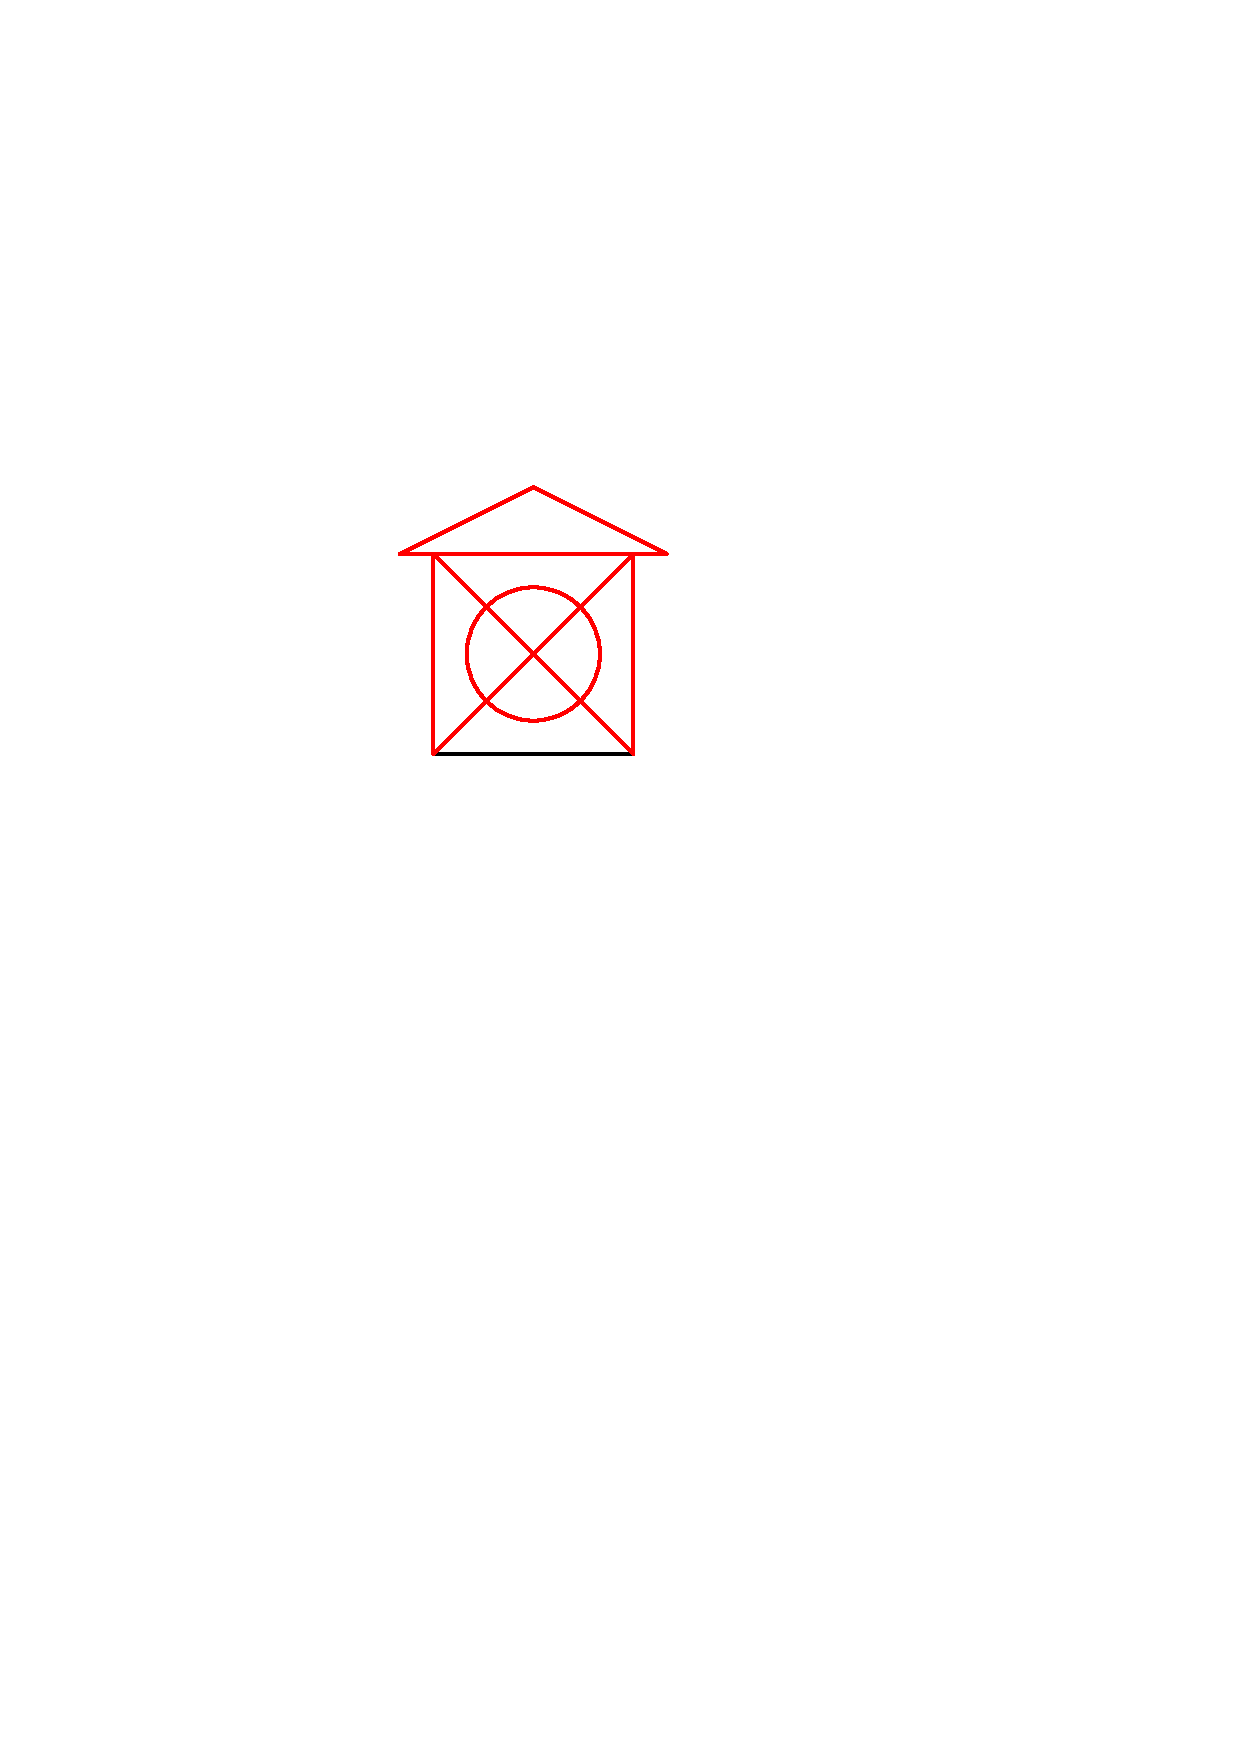
\includegraphics[width=0.25\linewidth]{house/house_pt11}
		\hspace{.05\linewidth}
		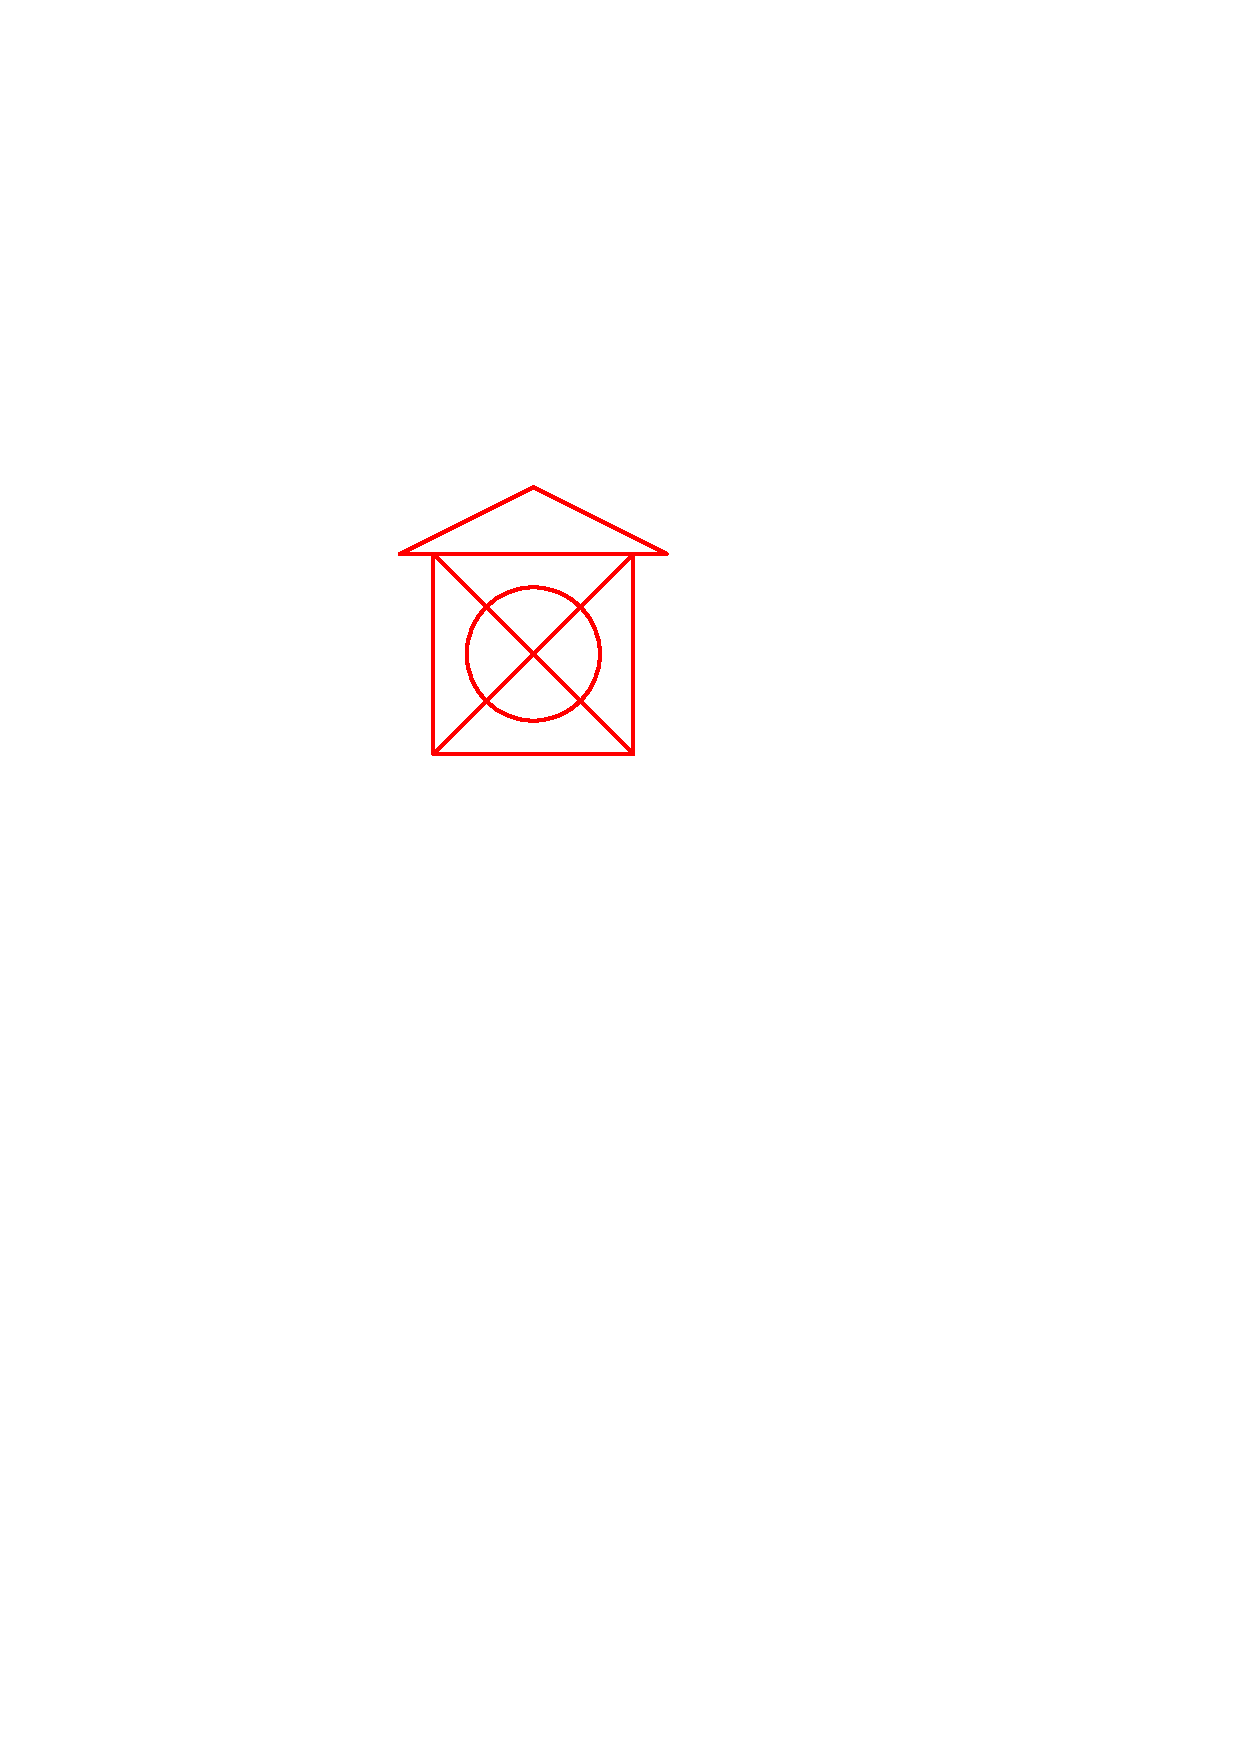
\includegraphics[width=0.25\linewidth]{house/house_pt12}
		\label{fig:housept1}
	\end{figure}
	
	\section{O Wolverine}
	
	Depois de duas folhas de tentativas chegou-se à conclusão que o problema é difícil de resolver \smiley{}. A principal reflexão é que nos casos onde houve maior aproximação de concluir o desafio sempre sobrava uma linha que para ser contornada iria exigir passar duas vezes pelo mesmo segmento, violando as regras estabelecidas.\\\vspace{1cm}
	
	\noindent\textit{Obs: A melhor justificativa nos casos que não resolvi é que aceito minha derrota depois de sucessivas tentativas!}
\end{document}